\documentclass[titlepage]{report}
\usepackage[BibLaTeX,noParIndent,InlineTodonotes]{multipack}

\title{Computational Materials Science - Molecular Dynamics}
\author{Schippers, C.F.}
\date{\today}


\begin{document}
\setAbstract{}
\inserttitletoc

\listoftodos
\newpage


\chapter{Theoretical exercises}
\section{Exercise 1}
A Gaussian polymer coil with $ N $ monomers with a distance $ a $ between each other has a mean square end-to-end distance $ \left\langle R^2 \right\rangle = a^2 N $ and an approximate volume $ V \sim \left\langle R^2 \right\rangle^{\frac{3}{2}} = a^3 N^{\frac{3}{2}} $ \parencite{Rubinstein2003}. The actual volume which is occupied by the monomers with volume $ v $ of the polymer is given by $ V\sub{pol} = v N $. The volume fraction $ \phi = \frac{V\sub{pol}}{V} $ is then given by
\begin{equation}
	\phi \sim \frac{v N}{a^3 N^{\frac{3}{2}}} = \frac{v}{a^3} N^{-\frac{1}{2}}.
\end{equation}

As two-particle interactions occur when one particles is found close to another, which has probability $ phi $, one can assume that $ \nu_2 $ scales as
\begin{equation}
	\nu_2 \sim N \phi \sim N^\frac{1}{2}.
\end{equation}

Analogous, three-particle interactions occur only when two particles are found close to another particle, which has probability $ \phi^2 $, one can assume that $ \nu_3 $ scales as
\begin{equation}
	\nu_3 \sim N \phi^2 \sim N^0.
\end{equation}

As one can see $ \nu_2 $ increases with increasing $ N $ so becomes a significant contribution for a polymer, whereas $ \nu_3 $ remains small as it does not depend on $ N $.

\section{Exercise 2}
\subsection{Exercise 2a}\label{subsec:THEX2a}
The Lennard-Jones potential is given by
\begin{equation}\label{eq:LennardJones}
	U = 4 \varepsilon \left[ \left(\frac{\sigma}{r}\right)^{12} - \left(\frac{\sigma}{r}\right)^6\right].
\end{equation}

To find the minimum of this potential, take the derivative to $ r $ and put to zero for $ r = r\sub{min} $
\begin{equation}
	\left. \pd{U}{r} \right|_{r=r\sub{min}} = 4 \varepsilon \left[ -12 \frac{\sigma^{12}}{r\sub{min}^{13}} + 6\frac{\sigma^{6}}{r\sub{min}^{7}} \right] = 0.
\end{equation}

This solves to
\begin{equation}
	r\sub{min} = \sqrt[6]{2} \sigma.
\end{equation}

Putting this in $ U $ gives
\begin{equation}
	U\left(r = r\sub{min}\right) = - \varepsilon.
\end{equation}

\subsection{Exercise 2b}
$ D_e $ is the depth of the potential well. 
A Taylor expansion of the potential around $ l - l_0 = 0 $ gives
\begin{subequations}
	\begin{align}
		v(l) =& D_e \left[ 1 - \exp\left(-a (l-l_0)\right) \right]^2 \\
		\approx& a^2 D_e (l-l_0)^2 + \mathcal{O}\left((l-l_0)^3\right).
	\end{align}
\end{subequations}
So at small deviations from $ l_0 $ the Morse potential is approximately equal to a harmonic potential $ v(l) = k/2 (l-l_0)^2 $ with $ k = 2 a^2 D_e $.
At distances away from the equilibrium the Morse potential deviates from the harmonic potential as the Morse potential approaches the potential depth $ D_e $ asymptotically. 
The Morse potential and the Taylor expansion around $ l - l_0 = 0 $ are shown in \cref{fig:THEX2b}.
\begin{figure}[h!]
	\centering
	% GNUPLOT: LaTeX picture with Postscript
\begingroup
  \makeatletter
  \providecommand\color[2][]{%
    \GenericError{(gnuplot) \space\space\space\@spaces}{%
      Package color not loaded in conjunction with
      terminal option `colourtext'%
    }{See the gnuplot documentation for explanation.%
    }{Either use 'blacktext' in gnuplot or load the package
      color.sty in LaTeX.}%
    \renewcommand\color[2][]{}%
  }%
  \providecommand\includegraphics[2][]{%
    \GenericError{(gnuplot) \space\space\space\@spaces}{%
      Package graphicx or graphics not loaded%
    }{See the gnuplot documentation for explanation.%
    }{The gnuplot epslatex terminal needs graphicx.sty or graphics.sty.}%
    \renewcommand\includegraphics[2][]{}%
  }%
  \providecommand\rotatebox[2]{#2}%
  \@ifundefined{ifGPcolor}{%
    \newif\ifGPcolor
    \GPcolorfalse
  }{}%
  \@ifundefined{ifGPblacktext}{%
    \newif\ifGPblacktext
    \GPblacktexttrue
  }{}%
  % define a \g@addto@macro without @ in the name:
  \let\gplgaddtomacro\g@addto@macro
  % define empty templates for all commands taking text:
  \gdef\gplbacktext{}%
  \gdef\gplfronttext{}%
  \makeatother
  \ifGPblacktext
    % no textcolor at all
    \def\colorrgb#1{}%
    \def\colorgray#1{}%
  \else
    % gray or color?
    \ifGPcolor
      \def\colorrgb#1{\color[rgb]{#1}}%
      \def\colorgray#1{\color[gray]{#1}}%
      \expandafter\def\csname LTw\endcsname{\color{white}}%
      \expandafter\def\csname LTb\endcsname{\color{black}}%
      \expandafter\def\csname LTa\endcsname{\color{black}}%
      \expandafter\def\csname LT0\endcsname{\color[rgb]{1,0,0}}%
      \expandafter\def\csname LT1\endcsname{\color[rgb]{0,1,0}}%
      \expandafter\def\csname LT2\endcsname{\color[rgb]{0,0,1}}%
      \expandafter\def\csname LT3\endcsname{\color[rgb]{1,0,1}}%
      \expandafter\def\csname LT4\endcsname{\color[rgb]{0,1,1}}%
      \expandafter\def\csname LT5\endcsname{\color[rgb]{1,1,0}}%
      \expandafter\def\csname LT6\endcsname{\color[rgb]{0,0,0}}%
      \expandafter\def\csname LT7\endcsname{\color[rgb]{1,0.3,0}}%
      \expandafter\def\csname LT8\endcsname{\color[rgb]{0.5,0.5,0.5}}%
    \else
      % gray
      \def\colorrgb#1{\color{black}}%
      \def\colorgray#1{\color[gray]{#1}}%
      \expandafter\def\csname LTw\endcsname{\color{white}}%
      \expandafter\def\csname LTb\endcsname{\color{black}}%
      \expandafter\def\csname LTa\endcsname{\color{black}}%
      \expandafter\def\csname LT0\endcsname{\color{black}}%
      \expandafter\def\csname LT1\endcsname{\color{black}}%
      \expandafter\def\csname LT2\endcsname{\color{black}}%
      \expandafter\def\csname LT3\endcsname{\color{black}}%
      \expandafter\def\csname LT4\endcsname{\color{black}}%
      \expandafter\def\csname LT5\endcsname{\color{black}}%
      \expandafter\def\csname LT6\endcsname{\color{black}}%
      \expandafter\def\csname LT7\endcsname{\color{black}}%
      \expandafter\def\csname LT8\endcsname{\color{black}}%
    \fi
  \fi
    \setlength{\unitlength}{0.0500bp}%
    \ifx\gptboxheight\undefined%
      \newlength{\gptboxheight}%
      \newlength{\gptboxwidth}%
      \newsavebox{\gptboxtext}%
    \fi%
    \setlength{\fboxrule}{0.5pt}%
    \setlength{\fboxsep}{1pt}%
\begin{picture}(8496.00,5040.00)%
    \gplgaddtomacro\gplbacktext{%
      \csname LTb\endcsname%
      \put(814,704){\makebox(0,0)[r]{\strut{}$0$}}%
      \put(814,1383){\makebox(0,0)[r]{\strut{}$0.5$}}%
      \put(814,2061){\makebox(0,0)[r]{\strut{}$1$}}%
      \put(814,2740){\makebox(0,0)[r]{\strut{}$1.5$}}%
      \put(814,3418){\makebox(0,0)[r]{\strut{}$2$}}%
      \put(814,4097){\makebox(0,0)[r]{\strut{}$2.5$}}%
      \put(814,4775){\makebox(0,0)[r]{\strut{}$3$}}%
      \put(946,484){\makebox(0,0){\strut{}$-2$}}%
      \put(2271,484){\makebox(0,0){\strut{}$0$}}%
      \put(3596,484){\makebox(0,0){\strut{}$2$}}%
      \put(4921,484){\makebox(0,0){\strut{}$4$}}%
      \put(6246,484){\makebox(0,0){\strut{}$6$}}%
      \put(7571,484){\makebox(0,0){\strut{}$8$}}%
      \put(7703,2061){\makebox(0,0)[l]{\strut{}$D_e$}}%
    }%
    \gplgaddtomacro\gplfronttext{%
      \csname LTb\endcsname%
      \put(176,2739){\rotatebox{-270}{\makebox(0,0){\strut{}$v/D_e$}}}%
      \put(4258,154){\makebox(0,0){\strut{}$a(l-l_0)$}}%
      \csname LTb\endcsname%
      \put(6584,4602){\makebox(0,0)[r]{\strut{}Morse potential}}%
      \csname LTb\endcsname%
      \put(6584,4382){\makebox(0,0)[r]{\strut{}Linearised potential}}%
    }%
    \gplbacktext
    \put(0,0){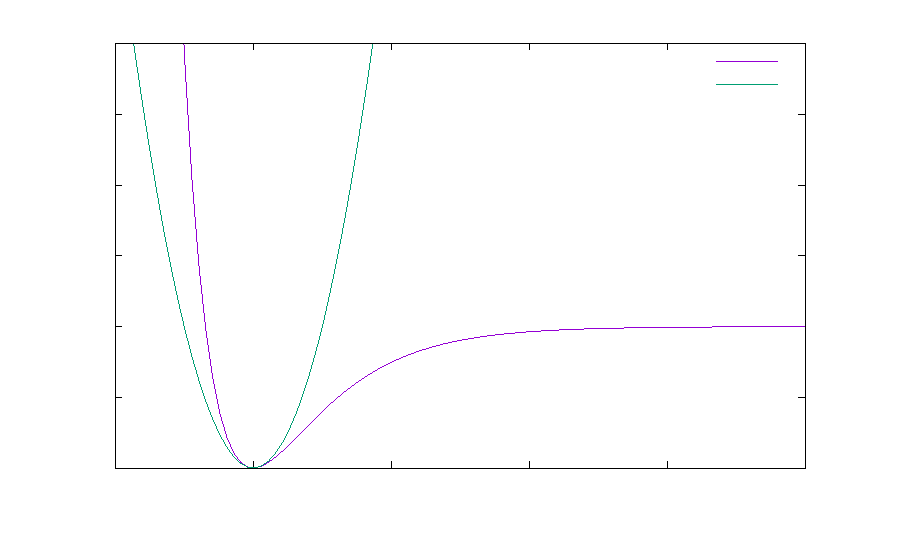
\includegraphics{THEX2b}}%
    \gplfronttext
  \end{picture}%
\endgroup

	\caption{Plot of the Morse potential and the Taylor expansion of the Morse potential around $ l-l_0 = 0 $.}
	\label{fig:THEX2b}
\end{figure}

\section{Exercise 3}
The characteristic frequency $ \omega $ of a harmonic spring with two masses is given by \cite[p. 164]{Taylor05}
\begin{equation}
	\omega = \sqrt{\frac{k\sub{spring}}{\mu}} 
\end{equation}
with $ k\sub{spring} $ the spring constant and $ \mu = \left(\frac{1}{m_1} + \frac{1}{m_2}\right)^{-1} $ the reduced mass. 
From this frequency, the wave-number $ k $ can be calculated with $ \omega = c k $, where $ c = 3\E{8}\unit{m \, s^{-1}} $ is the speed of light. This results in the values found in \cref{tab:THEX3wavenumbers}.
% Using $ 1\unit{N/m} = 1.4393 \unit{kcal \, mol^{-1} \textrm{\AA}^{-2}} $ and..
\begin{table}[h!]
	\centering
	\caption{Wave-numbers in $ \unit{cm^{-1}} $ for various bonds.}
	\label{tab:THEX3wavenumbers}
	\begin{tabular}{lr}
		Bond & Wave-number ($\unit{cm^{-1}}$) \\ 
		C-C & 4955.33 \\ 
		C=C & 7310.84 \\ 
		C=0 & 7257.00
	\end{tabular} 
\end{table}

\section{Exercise 4}
The total amount of boxes that has to be taken into account in $ N $-dimensions scales as $ C^N $.
For $ 1D $ systems this is known to be $ 3 $, for $ 2D $ systems this is $ 9 $ and for $ 3D $ systems this is $ 27 $, which leads to $ C=3 $.
So in a $ N $ dimensions the amount of periodic images is given by $ 3^N - 1 $.

\section{Exercise 5}
Using $ \vec{F} = m \ddot{\vec{r}} $, the virial $ \langle G \rangle $ can be calculated as
\begin{subequations}
	\begin{align}
		\langle G \rangle =& \left\langle \sum_i \vec{r}_i \cdot \vec{F}_i \right\rangle\\
		=& m \left\langle \sum_i \vec{r}_i \cdot \ddot{\vec{r}}_i \right\rangle.
	\end{align}
\end{subequations}

The average can be calculated using equation 2.1 from the lecture notes:
\begin{subequations}
	\begin{align}
	\langle G \rangle =& \lim\limits_{t\sub{obs} \rightarrow \infty} \frac{1}{t\sub{obs}} \int_{0}^{t\sub{obs}} m \sum_i \vec{r}_i \cdot \ddot{\vec{r}}_i \d t\\
	=& \lim\limits_{t\sub{obs} \rightarrow \infty} \frac{m}{t\sub{obs}} \left( \left. \left[\sum_i \vec{r}_i \cdot \dot{\vec{r}}_i \right] \right|_0^{t\sub{obs}} - \int_{0}^{t\sub{obs}} \sum_i \dot{\vec{r}}_i \cdot \dot{\vec{r}}_i \d t \right).
	\end{align}
\end{subequations}

As the first term vanishes as it is divided by $ t\sub{obs} $, which goes to $ \infty $. By using equation 2.1 from the lecture notes and $ \sum_i \left\langle \dot{\vec{r}}_i^{\;2} \right\rangle = N \left\langle \dot{\vec{r}}^{\;2} \right\rangle $, the remaining part can be rewritten:
\begin{subequations}
	\begin{align}
	\langle G \rangle =& - \lim\limits_{t\sub{obs} \rightarrow \infty} \frac{m}{t\sub{obs}} \int_{0}^{t\sub{obs}} \sum_i \dot{\vec{r}}_i^{\;2} \d t \\
	=& -m \left\langle \sum_i \dot{\vec{r}}_i^{\;2} \right\rangle\\
	=& -m N \left\langle \dot{\vec{r}}^{\;2} \right\rangle.
	\end{align}
\end{subequations}

As according to the equipartition theorem $ 3 k\sub{B} T = m \left\langle \vec{v}^{\;2} \right\rangle = m \left\langle \dot{\vec{r}}^{\;2} \right\rangle $, the virial is given by $ \langle G \rangle = -3 n k\sub{B} T $.\\

Moreover, the sum $ \sum_i \vec{r} \cdot \vec{F}_i\suprm{ext} $ can be calculated using $ \d \vec{F}_i\suprm{ext} = - P \d \vec{A})_i $:
\begin{subequations}
	\begin{align}
		\sum_i \vec{r} \cdot \vec{F}_i\suprm{ext} =& \sum_i \int \vec{r} \cdot \vec{F}_i\suprm{ext}\\
		=& \sum_i \int_{A_i} P \vec{r} \cdot \d\vec{A}_i.
	\end{align}
\end{subequations}

Using the Gauss theorem and the fact that $ \nabla \vec{r} = 3 $ this can be further calculated as
\begin{subequations}
	\begin{align}
		\sum_i \int_{A_i} P \vec{r} \cdot \d\vec{A}_i =& -P \sum_i \int_{V_i} \nabla \cdot \vec{r}_i \d V_i\\
		=& -3 P \sum_i V_i\\
		=& -3 P V.
	\end{align}
\end{subequations}

This results can be combined with $ \langle G \rangle = -3 n k\sub{B} T $ using $ \vec{F} = \vec{F}\suprm{int} + \vec{F}\suprm{ext} $:

\begin{subequations}
	\begin{align}
		-3 V P = \sum_i \vec{r} \cdot \vec{F}_i\suprm{ext} =& \left\langle \sum_i \vec{r}_i \cdot \vec{F}_i \right\rangle - \left\langle \sum_i \vec{r}_i \cdot \vec{F}_i\suprm{int} \right\rangle\\
		=& \langle G \rangle - \left\langle \sum_i \vec{r}_i \cdot \vec{F}_i\suprm{int} \right\rangle\\
		=& -3 N K\sub{B} T - \left\langle \sum_i \vec{r}_i \cdot \vec{F}_i\suprm{int} \right\rangle.
	\end{align}
\end{subequations}

This yields
\begin{equation}
P = \frac{1}{V} \left( N k\sub{B} T + \frac{1}{3} \left\langle \sum_i \vec{r}_i \cdot \vec{F}_i\suprm{int} \right\rangle \right).
\end{equation}

\section{Exercise 6}
\subsection{Exercise 6a}
The magnitude of the barrier separating trans and gauche isomeric states for polyethylene is $ 14 \unit{kJ / mol} $, which is equal to $ 5.65 k\sub{B} T $.

\subsection{Exercise 6b}
The Lennard-Jones time is defined as $ \tau\sub{LJ} = a\sqrt{\frac{m}{\varepsilon}} $.
For the specified model, $ a = 1 \AA $ is the size of the particle, $ m = 12 a.u. = 1.992 \E{-28} \unit{kg} $ is the mass and $ \varepsilon = 0.5 \unit{kJ / moll} = 8.3 \E{-20} \unit{J} $ is the interaction energy, so the Lennard-Jones time is given by $ \tau\sub{LJ} \approx 10^{-10} \sqrt{\frac{1.992 \E{-28}}{8.3 \E{-20}}} \approx 0.5 \unit{ps} $.
The rotational diffusion time is defined as $ \tau\sub{diff} = \frac{8 \pi \eta (l/2)^3}{k\sub{B} T} $.
With viscosity $ \eta = 1 \unit{mPa \, s} $ and temperature $ T = 300 \unit{K} $ and length $ l = 1 \AA $, this gives $ \tau\sub{diff} = \frac{8 \pi \E{-3} \E{-30}}{4.11\E{-21}} \approx 6\unit{ps} $.
An appropriate time-step would be $ \Delta t = \tau\sub{LJ} / 100 = 5 \E{-3} \unit{ps} $, as the Lennard-Jones time is the shortest time-scale. 

\section{Exercise 7}
The kinetic energy $ E\sub{k} $ and it's time derivative are given by
\begin{subequations}
	\begin{align}
		E\sub{k} =& \sum_{1=i}^{3N}\frac{1}{2} m_i v_i^2\\
		\dd{E\sub{k}}{t} =& \sum_{1=i}^{3N} m_i \dot{v}_i v_i.
	\end{align}
\end{subequations}

Using $	m_i \dot{v}_i = F_i + m_i \gamma \left(\frac{T_0}{T} -1 \right) v_i $, this can be written as
\begin{subequations}
	\begin{align}
		\dd{E\sub{k}}{t} =& \sum_{1=i}^{3N} \left( v_i F_i + m_i \gamma \left(\frac{T_0}{T} -1 \right) v_i^2 \right)\\
		=& \sum_{1=i}^{3N} v_i F_i + \gamma \left(\frac{T_0}{T} -1 \right) 2 E\sub{k}.
	\end{align}
\end{subequations}

Now using $ E\sub{k} = \frac{3}{2}N k\sub{B} T $ one can write
\begin{equation}
	\dd{E\sub{k}}{t} = \sum_{1=i}^{3N} v_i F_i + 2\gamma \left(\frac{3 N}{2} k\sub{B} T_0 - E\sub{k} \right).
\end{equation}


\chapter{Molecular Dynamics of a Simple Liquid}

\section{Exercise 1}
The model parameters are set in de main function.
The masses of the particles are determined by the variable \texttt{special}.
If $ \texttt{special} = 1 $ the particles have mass 1, but if $ \texttt{special} \neq 1 $ the particles have random masses following a Gaussian distribution centred around 1.

\section{Exercise 2}
\subsection{Exercise 2a}
The Lennard-Jones potential decreases sharply for values smaller than $ r\sub{min} = \sqrt[6]{2}\sigma \approx 1.122 \sigma $ and therefore induces a strong repulsive force, as can be seen in \cref{fig:MDSLEX2b}.
particles are initially spaced less then this $ r\sub{min} $, this force might cause particles to be displaced a multiple of the box size, which is unrealistic and thus leads to unrealistic behaviour.
Therefore, a spacing of $ r = 1.2 \sigma $ is a reasonable choice.

\subsection{Exercise 2b}
The Lennard-Jones potential is plotted in \cref{fig:MDSLEX2b}.
The minimum of the potential is $ U(r\sub{min}) = -\varepsilon $ with $ r\sub{min} = \sqrt[6]{2} \sigma $ as was calculated in theoretical exercise 2a (\cref{subsec:THEX2a}).
The asymptote for $ r \rightarrow 0 $ is $ U(r \rightarrow 0) \rightarrow \infty $ and the asymptote for $ r \rightarrow \infty $ is $ U(r \rightarrow \infty) \rightarrow 0 $.

\begin{figure}[h!]
	\centering
	%% Creator: Matplotlib, PGF backend
%%
%% To include the figure in your LaTeX document, write
%%   \input{<filename>.pgf}
%%
%% Make sure the required packages are loaded in your preamble
%%   \usepackage{pgf}
%%
%% Figures using additional raster images can only be included by \input if
%% they are in the same directory as the main LaTeX file. For loading figures
%% from other directories you can use the `import` package
%%   \usepackage{import}
%% and then include the figures with
%%   \import{<path to file>}{<filename>.pgf}
%%
%% Matplotlib used the following preamble
%%   \usepackage[utf8x]{inputenc}
%%   \usepackage[T1]{fontenc}
%%
\begingroup%
\makeatletter%
\begin{pgfpicture}%
\pgfpathrectangle{\pgfpointorigin}{\pgfqpoint{4.133858in}{2.480315in}}%
\pgfusepath{use as bounding box, clip}%
\begin{pgfscope}%
\pgfsetbuttcap%
\pgfsetmiterjoin%
\definecolor{currentfill}{rgb}{1.000000,1.000000,1.000000}%
\pgfsetfillcolor{currentfill}%
\pgfsetlinewidth{0.000000pt}%
\definecolor{currentstroke}{rgb}{1.000000,1.000000,1.000000}%
\pgfsetstrokecolor{currentstroke}%
\pgfsetdash{}{0pt}%
\pgfpathmoveto{\pgfqpoint{0.000000in}{0.000000in}}%
\pgfpathlineto{\pgfqpoint{4.133858in}{0.000000in}}%
\pgfpathlineto{\pgfqpoint{4.133858in}{2.480315in}}%
\pgfpathlineto{\pgfqpoint{0.000000in}{2.480315in}}%
\pgfpathclose%
\pgfusepath{fill}%
\end{pgfscope}%
\begin{pgfscope}%
\pgfsetbuttcap%
\pgfsetmiterjoin%
\definecolor{currentfill}{rgb}{1.000000,1.000000,1.000000}%
\pgfsetfillcolor{currentfill}%
\pgfsetlinewidth{0.000000pt}%
\definecolor{currentstroke}{rgb}{0.000000,0.000000,0.000000}%
\pgfsetstrokecolor{currentstroke}%
\pgfsetstrokeopacity{0.000000}%
\pgfsetdash{}{0pt}%
\pgfpathmoveto{\pgfqpoint{0.564740in}{0.512013in}}%
\pgfpathlineto{\pgfqpoint{3.908433in}{0.512013in}}%
\pgfpathlineto{\pgfqpoint{3.908433in}{2.281253in}}%
\pgfpathlineto{\pgfqpoint{0.564740in}{2.281253in}}%
\pgfpathclose%
\pgfusepath{fill}%
\end{pgfscope}%
\begin{pgfscope}%
\pgfpathrectangle{\pgfqpoint{0.564740in}{0.512013in}}{\pgfqpoint{3.343693in}{1.769240in}} %
\pgfusepath{clip}%
\pgfsetrectcap%
\pgfsetroundjoin%
\pgfsetlinewidth{1.003750pt}%
\definecolor{currentstroke}{rgb}{0.000000,0.000000,1.000000}%
\pgfsetstrokecolor{currentstroke}%
\pgfsetdash{}{0pt}%
\pgfpathmoveto{\pgfqpoint{1.582656in}{2.281753in}}%
\pgfpathlineto{\pgfqpoint{1.591254in}{2.059304in}}%
\pgfpathlineto{\pgfqpoint{1.602399in}{1.815961in}}%
\pgfpathlineto{\pgfqpoint{1.613545in}{1.610817in}}%
\pgfpathlineto{\pgfqpoint{1.624691in}{1.438101in}}%
\pgfpathlineto{\pgfqpoint{1.635836in}{1.292930in}}%
\pgfpathlineto{\pgfqpoint{1.646982in}{1.171169in}}%
\pgfpathlineto{\pgfqpoint{1.658127in}{1.069309in}}%
\pgfpathlineto{\pgfqpoint{1.669273in}{0.984373in}}%
\pgfpathlineto{\pgfqpoint{1.680419in}{0.913828in}}%
\pgfpathlineto{\pgfqpoint{1.691564in}{0.855523in}}%
\pgfpathlineto{\pgfqpoint{1.702710in}{0.807623in}}%
\pgfpathlineto{\pgfqpoint{1.713856in}{0.768567in}}%
\pgfpathlineto{\pgfqpoint{1.725001in}{0.737022in}}%
\pgfpathlineto{\pgfqpoint{1.736147in}{0.711853in}}%
\pgfpathlineto{\pgfqpoint{1.747293in}{0.692088in}}%
\pgfpathlineto{\pgfqpoint{1.758438in}{0.676900in}}%
\pgfpathlineto{\pgfqpoint{1.769584in}{0.665581in}}%
\pgfpathlineto{\pgfqpoint{1.780730in}{0.657524in}}%
\pgfpathlineto{\pgfqpoint{1.791875in}{0.652214in}}%
\pgfpathlineto{\pgfqpoint{1.803021in}{0.649207in}}%
\pgfpathlineto{\pgfqpoint{1.814166in}{0.648125in}}%
\pgfpathlineto{\pgfqpoint{1.825312in}{0.648646in}}%
\pgfpathlineto{\pgfqpoint{1.836458in}{0.650494in}}%
\pgfpathlineto{\pgfqpoint{1.847603in}{0.653431in}}%
\pgfpathlineto{\pgfqpoint{1.858749in}{0.657259in}}%
\pgfpathlineto{\pgfqpoint{1.869895in}{0.661804in}}%
\pgfpathlineto{\pgfqpoint{1.881040in}{0.666920in}}%
\pgfpathlineto{\pgfqpoint{1.892186in}{0.672484in}}%
\pgfpathlineto{\pgfqpoint{1.903332in}{0.678390in}}%
\pgfpathlineto{\pgfqpoint{1.914477in}{0.684548in}}%
\pgfpathlineto{\pgfqpoint{1.925623in}{0.690883in}}%
\pgfpathlineto{\pgfqpoint{1.947914in}{0.703837in}}%
\pgfpathlineto{\pgfqpoint{1.970205in}{0.716855in}}%
\pgfpathlineto{\pgfqpoint{1.981351in}{0.723299in}}%
\pgfpathlineto{\pgfqpoint{1.992497in}{0.729663in}}%
\pgfpathlineto{\pgfqpoint{2.003642in}{0.735927in}}%
\pgfpathlineto{\pgfqpoint{2.014788in}{0.742074in}}%
\pgfpathlineto{\pgfqpoint{2.025934in}{0.748091in}}%
\pgfpathlineto{\pgfqpoint{2.037079in}{0.753968in}}%
\pgfpathlineto{\pgfqpoint{2.048225in}{0.759696in}}%
\pgfpathlineto{\pgfqpoint{2.059371in}{0.765271in}}%
\pgfpathlineto{\pgfqpoint{2.070516in}{0.770687in}}%
\pgfpathlineto{\pgfqpoint{2.081662in}{0.775943in}}%
\pgfpathlineto{\pgfqpoint{2.092808in}{0.781038in}}%
\pgfpathlineto{\pgfqpoint{2.103953in}{0.785972in}}%
\pgfpathlineto{\pgfqpoint{2.115099in}{0.790745in}}%
\pgfpathlineto{\pgfqpoint{2.126245in}{0.795359in}}%
\pgfpathlineto{\pgfqpoint{2.137390in}{0.799816in}}%
\pgfpathlineto{\pgfqpoint{2.148536in}{0.804120in}}%
\pgfpathlineto{\pgfqpoint{2.159681in}{0.808272in}}%
\pgfpathlineto{\pgfqpoint{2.170827in}{0.812277in}}%
\pgfpathlineto{\pgfqpoint{2.181973in}{0.816138in}}%
\pgfpathlineto{\pgfqpoint{2.193118in}{0.819859in}}%
\pgfpathlineto{\pgfqpoint{2.204264in}{0.823443in}}%
\pgfpathlineto{\pgfqpoint{2.215410in}{0.826896in}}%
\pgfpathlineto{\pgfqpoint{2.226555in}{0.830221in}}%
\pgfpathlineto{\pgfqpoint{2.237701in}{0.833421in}}%
\pgfpathlineto{\pgfqpoint{2.248847in}{0.836502in}}%
\pgfpathlineto{\pgfqpoint{2.259992in}{0.839467in}}%
\pgfpathlineto{\pgfqpoint{2.271138in}{0.842320in}}%
\pgfpathlineto{\pgfqpoint{2.282284in}{0.845066in}}%
\pgfpathlineto{\pgfqpoint{2.293429in}{0.847707in}}%
\pgfpathlineto{\pgfqpoint{2.304575in}{0.850249in}}%
\pgfpathlineto{\pgfqpoint{2.315720in}{0.852694in}}%
\pgfpathlineto{\pgfqpoint{2.326866in}{0.855046in}}%
\pgfpathlineto{\pgfqpoint{2.338012in}{0.857309in}}%
\pgfpathlineto{\pgfqpoint{2.349157in}{0.859486in}}%
\pgfpathlineto{\pgfqpoint{2.360303in}{0.861580in}}%
\pgfpathlineto{\pgfqpoint{2.371449in}{0.863595in}}%
\pgfpathlineto{\pgfqpoint{2.382594in}{0.865534in}}%
\pgfpathlineto{\pgfqpoint{2.393740in}{0.867400in}}%
\pgfpathlineto{\pgfqpoint{2.404886in}{0.869195in}}%
\pgfpathlineto{\pgfqpoint{2.416031in}{0.870922in}}%
\pgfpathlineto{\pgfqpoint{2.427177in}{0.872585in}}%
\pgfpathlineto{\pgfqpoint{2.438323in}{0.874185in}}%
\pgfpathlineto{\pgfqpoint{2.449468in}{0.875725in}}%
\pgfpathlineto{\pgfqpoint{2.471759in}{0.878634in}}%
\pgfpathlineto{\pgfqpoint{2.494051in}{0.881332in}}%
\pgfpathlineto{\pgfqpoint{2.516342in}{0.883834in}}%
\pgfpathlineto{\pgfqpoint{2.538633in}{0.886155in}}%
\pgfpathlineto{\pgfqpoint{2.560925in}{0.888310in}}%
\pgfpathlineto{\pgfqpoint{2.583216in}{0.890312in}}%
\pgfpathlineto{\pgfqpoint{2.605507in}{0.892172in}}%
\pgfpathlineto{\pgfqpoint{2.627798in}{0.893902in}}%
\pgfpathlineto{\pgfqpoint{2.650090in}{0.895511in}}%
\pgfpathlineto{\pgfqpoint{2.672381in}{0.897009in}}%
\pgfpathlineto{\pgfqpoint{2.694672in}{0.898404in}}%
\pgfpathlineto{\pgfqpoint{2.716964in}{0.899703in}}%
\pgfpathlineto{\pgfqpoint{2.739255in}{0.900915in}}%
\pgfpathlineto{\pgfqpoint{2.761546in}{0.902046in}}%
\pgfpathlineto{\pgfqpoint{2.794983in}{0.903603in}}%
\pgfpathlineto{\pgfqpoint{2.828420in}{0.905008in}}%
\pgfpathlineto{\pgfqpoint{2.861857in}{0.906279in}}%
\pgfpathlineto{\pgfqpoint{2.895294in}{0.907429in}}%
\pgfpathlineto{\pgfqpoint{2.928731in}{0.908472in}}%
\pgfpathlineto{\pgfqpoint{2.962168in}{0.909418in}}%
\pgfpathlineto{\pgfqpoint{3.006750in}{0.910546in}}%
\pgfpathlineto{\pgfqpoint{3.051333in}{0.911541in}}%
\pgfpathlineto{\pgfqpoint{3.095915in}{0.912421in}}%
\pgfpathlineto{\pgfqpoint{3.140498in}{0.913199in}}%
\pgfpathlineto{\pgfqpoint{3.196226in}{0.914050in}}%
\pgfpathlineto{\pgfqpoint{3.251954in}{0.914784in}}%
\pgfpathlineto{\pgfqpoint{3.318828in}{0.915537in}}%
\pgfpathlineto{\pgfqpoint{3.385702in}{0.916173in}}%
\pgfpathlineto{\pgfqpoint{3.463722in}{0.916794in}}%
\pgfpathlineto{\pgfqpoint{3.552887in}{0.917375in}}%
\pgfpathlineto{\pgfqpoint{3.653198in}{0.917900in}}%
\pgfpathlineto{\pgfqpoint{3.764654in}{0.918359in}}%
\pgfpathlineto{\pgfqpoint{3.887256in}{0.918750in}}%
\pgfpathlineto{\pgfqpoint{3.898402in}{0.918781in}}%
\pgfpathlineto{\pgfqpoint{3.898402in}{0.918781in}}%
\pgfusepath{stroke}%
\end{pgfscope}%
\begin{pgfscope}%
\pgfsetrectcap%
\pgfsetmiterjoin%
\pgfsetlinewidth{1.003750pt}%
\definecolor{currentstroke}{rgb}{0.000000,0.000000,0.000000}%
\pgfsetstrokecolor{currentstroke}%
\pgfsetdash{}{0pt}%
\pgfpathmoveto{\pgfqpoint{0.564740in}{2.281253in}}%
\pgfpathlineto{\pgfqpoint{3.908433in}{2.281253in}}%
\pgfusepath{stroke}%
\end{pgfscope}%
\begin{pgfscope}%
\pgfsetrectcap%
\pgfsetmiterjoin%
\pgfsetlinewidth{1.003750pt}%
\definecolor{currentstroke}{rgb}{0.000000,0.000000,0.000000}%
\pgfsetstrokecolor{currentstroke}%
\pgfsetdash{}{0pt}%
\pgfpathmoveto{\pgfqpoint{0.564740in}{0.512013in}}%
\pgfpathlineto{\pgfqpoint{3.908433in}{0.512013in}}%
\pgfusepath{stroke}%
\end{pgfscope}%
\begin{pgfscope}%
\pgfsetrectcap%
\pgfsetmiterjoin%
\pgfsetlinewidth{1.003750pt}%
\definecolor{currentstroke}{rgb}{0.000000,0.000000,0.000000}%
\pgfsetstrokecolor{currentstroke}%
\pgfsetdash{}{0pt}%
\pgfpathmoveto{\pgfqpoint{3.908433in}{0.512013in}}%
\pgfpathlineto{\pgfqpoint{3.908433in}{2.281253in}}%
\pgfusepath{stroke}%
\end{pgfscope}%
\begin{pgfscope}%
\pgfsetrectcap%
\pgfsetmiterjoin%
\pgfsetlinewidth{1.003750pt}%
\definecolor{currentstroke}{rgb}{0.000000,0.000000,0.000000}%
\pgfsetstrokecolor{currentstroke}%
\pgfsetdash{}{0pt}%
\pgfpathmoveto{\pgfqpoint{0.564740in}{0.512013in}}%
\pgfpathlineto{\pgfqpoint{0.564740in}{2.281253in}}%
\pgfusepath{stroke}%
\end{pgfscope}%
\begin{pgfscope}%
\pgfsetbuttcap%
\pgfsetroundjoin%
\definecolor{currentfill}{rgb}{0.000000,0.000000,0.000000}%
\pgfsetfillcolor{currentfill}%
\pgfsetlinewidth{0.501875pt}%
\definecolor{currentstroke}{rgb}{0.000000,0.000000,0.000000}%
\pgfsetstrokecolor{currentstroke}%
\pgfsetdash{}{0pt}%
\pgfsys@defobject{currentmarker}{\pgfqpoint{0.000000in}{0.000000in}}{\pgfqpoint{0.000000in}{0.055556in}}{%
\pgfpathmoveto{\pgfqpoint{0.000000in}{0.000000in}}%
\pgfpathlineto{\pgfqpoint{0.000000in}{0.055556in}}%
\pgfusepath{stroke,fill}%
}%
\begin{pgfscope}%
\pgfsys@transformshift{0.564740in}{0.512013in}%
\pgfsys@useobject{currentmarker}{}%
\end{pgfscope}%
\end{pgfscope}%
\begin{pgfscope}%
\pgfsetbuttcap%
\pgfsetroundjoin%
\definecolor{currentfill}{rgb}{0.000000,0.000000,0.000000}%
\pgfsetfillcolor{currentfill}%
\pgfsetlinewidth{0.501875pt}%
\definecolor{currentstroke}{rgb}{0.000000,0.000000,0.000000}%
\pgfsetstrokecolor{currentstroke}%
\pgfsetdash{}{0pt}%
\pgfsys@defobject{currentmarker}{\pgfqpoint{0.000000in}{-0.055556in}}{\pgfqpoint{0.000000in}{0.000000in}}{%
\pgfpathmoveto{\pgfqpoint{0.000000in}{0.000000in}}%
\pgfpathlineto{\pgfqpoint{0.000000in}{-0.055556in}}%
\pgfusepath{stroke,fill}%
}%
\begin{pgfscope}%
\pgfsys@transformshift{0.564740in}{2.281253in}%
\pgfsys@useobject{currentmarker}{}%
\end{pgfscope}%
\end{pgfscope}%
\begin{pgfscope}%
\pgftext[x=0.564740in,y=0.456458in,,top]{\rmfamily\fontsize{8.000000}{9.600000}\selectfont \(\displaystyle 0.0\)}%
\end{pgfscope}%
\begin{pgfscope}%
\pgfsetbuttcap%
\pgfsetroundjoin%
\definecolor{currentfill}{rgb}{0.000000,0.000000,0.000000}%
\pgfsetfillcolor{currentfill}%
\pgfsetlinewidth{0.501875pt}%
\definecolor{currentstroke}{rgb}{0.000000,0.000000,0.000000}%
\pgfsetstrokecolor{currentstroke}%
\pgfsetdash{}{0pt}%
\pgfsys@defobject{currentmarker}{\pgfqpoint{0.000000in}{0.000000in}}{\pgfqpoint{0.000000in}{0.055556in}}{%
\pgfpathmoveto{\pgfqpoint{0.000000in}{0.000000in}}%
\pgfpathlineto{\pgfqpoint{0.000000in}{0.055556in}}%
\pgfusepath{stroke,fill}%
}%
\begin{pgfscope}%
\pgfsys@transformshift{1.122022in}{0.512013in}%
\pgfsys@useobject{currentmarker}{}%
\end{pgfscope}%
\end{pgfscope}%
\begin{pgfscope}%
\pgfsetbuttcap%
\pgfsetroundjoin%
\definecolor{currentfill}{rgb}{0.000000,0.000000,0.000000}%
\pgfsetfillcolor{currentfill}%
\pgfsetlinewidth{0.501875pt}%
\definecolor{currentstroke}{rgb}{0.000000,0.000000,0.000000}%
\pgfsetstrokecolor{currentstroke}%
\pgfsetdash{}{0pt}%
\pgfsys@defobject{currentmarker}{\pgfqpoint{0.000000in}{-0.055556in}}{\pgfqpoint{0.000000in}{0.000000in}}{%
\pgfpathmoveto{\pgfqpoint{0.000000in}{0.000000in}}%
\pgfpathlineto{\pgfqpoint{0.000000in}{-0.055556in}}%
\pgfusepath{stroke,fill}%
}%
\begin{pgfscope}%
\pgfsys@transformshift{1.122022in}{2.281253in}%
\pgfsys@useobject{currentmarker}{}%
\end{pgfscope}%
\end{pgfscope}%
\begin{pgfscope}%
\pgftext[x=1.122022in,y=0.456458in,,top]{\rmfamily\fontsize{8.000000}{9.600000}\selectfont \(\displaystyle 0.5\)}%
\end{pgfscope}%
\begin{pgfscope}%
\pgfsetbuttcap%
\pgfsetroundjoin%
\definecolor{currentfill}{rgb}{0.000000,0.000000,0.000000}%
\pgfsetfillcolor{currentfill}%
\pgfsetlinewidth{0.501875pt}%
\definecolor{currentstroke}{rgb}{0.000000,0.000000,0.000000}%
\pgfsetstrokecolor{currentstroke}%
\pgfsetdash{}{0pt}%
\pgfsys@defobject{currentmarker}{\pgfqpoint{0.000000in}{0.000000in}}{\pgfqpoint{0.000000in}{0.055556in}}{%
\pgfpathmoveto{\pgfqpoint{0.000000in}{0.000000in}}%
\pgfpathlineto{\pgfqpoint{0.000000in}{0.055556in}}%
\pgfusepath{stroke,fill}%
}%
\begin{pgfscope}%
\pgfsys@transformshift{1.679304in}{0.512013in}%
\pgfsys@useobject{currentmarker}{}%
\end{pgfscope}%
\end{pgfscope}%
\begin{pgfscope}%
\pgfsetbuttcap%
\pgfsetroundjoin%
\definecolor{currentfill}{rgb}{0.000000,0.000000,0.000000}%
\pgfsetfillcolor{currentfill}%
\pgfsetlinewidth{0.501875pt}%
\definecolor{currentstroke}{rgb}{0.000000,0.000000,0.000000}%
\pgfsetstrokecolor{currentstroke}%
\pgfsetdash{}{0pt}%
\pgfsys@defobject{currentmarker}{\pgfqpoint{0.000000in}{-0.055556in}}{\pgfqpoint{0.000000in}{0.000000in}}{%
\pgfpathmoveto{\pgfqpoint{0.000000in}{0.000000in}}%
\pgfpathlineto{\pgfqpoint{0.000000in}{-0.055556in}}%
\pgfusepath{stroke,fill}%
}%
\begin{pgfscope}%
\pgfsys@transformshift{1.679304in}{2.281253in}%
\pgfsys@useobject{currentmarker}{}%
\end{pgfscope}%
\end{pgfscope}%
\begin{pgfscope}%
\pgftext[x=1.679304in,y=0.456458in,,top]{\rmfamily\fontsize{8.000000}{9.600000}\selectfont \(\displaystyle 1.0\)}%
\end{pgfscope}%
\begin{pgfscope}%
\pgfsetbuttcap%
\pgfsetroundjoin%
\definecolor{currentfill}{rgb}{0.000000,0.000000,0.000000}%
\pgfsetfillcolor{currentfill}%
\pgfsetlinewidth{0.501875pt}%
\definecolor{currentstroke}{rgb}{0.000000,0.000000,0.000000}%
\pgfsetstrokecolor{currentstroke}%
\pgfsetdash{}{0pt}%
\pgfsys@defobject{currentmarker}{\pgfqpoint{0.000000in}{0.000000in}}{\pgfqpoint{0.000000in}{0.055556in}}{%
\pgfpathmoveto{\pgfqpoint{0.000000in}{0.000000in}}%
\pgfpathlineto{\pgfqpoint{0.000000in}{0.055556in}}%
\pgfusepath{stroke,fill}%
}%
\begin{pgfscope}%
\pgfsys@transformshift{2.236586in}{0.512013in}%
\pgfsys@useobject{currentmarker}{}%
\end{pgfscope}%
\end{pgfscope}%
\begin{pgfscope}%
\pgfsetbuttcap%
\pgfsetroundjoin%
\definecolor{currentfill}{rgb}{0.000000,0.000000,0.000000}%
\pgfsetfillcolor{currentfill}%
\pgfsetlinewidth{0.501875pt}%
\definecolor{currentstroke}{rgb}{0.000000,0.000000,0.000000}%
\pgfsetstrokecolor{currentstroke}%
\pgfsetdash{}{0pt}%
\pgfsys@defobject{currentmarker}{\pgfqpoint{0.000000in}{-0.055556in}}{\pgfqpoint{0.000000in}{0.000000in}}{%
\pgfpathmoveto{\pgfqpoint{0.000000in}{0.000000in}}%
\pgfpathlineto{\pgfqpoint{0.000000in}{-0.055556in}}%
\pgfusepath{stroke,fill}%
}%
\begin{pgfscope}%
\pgfsys@transformshift{2.236586in}{2.281253in}%
\pgfsys@useobject{currentmarker}{}%
\end{pgfscope}%
\end{pgfscope}%
\begin{pgfscope}%
\pgftext[x=2.236586in,y=0.456458in,,top]{\rmfamily\fontsize{8.000000}{9.600000}\selectfont \(\displaystyle 1.5\)}%
\end{pgfscope}%
\begin{pgfscope}%
\pgfsetbuttcap%
\pgfsetroundjoin%
\definecolor{currentfill}{rgb}{0.000000,0.000000,0.000000}%
\pgfsetfillcolor{currentfill}%
\pgfsetlinewidth{0.501875pt}%
\definecolor{currentstroke}{rgb}{0.000000,0.000000,0.000000}%
\pgfsetstrokecolor{currentstroke}%
\pgfsetdash{}{0pt}%
\pgfsys@defobject{currentmarker}{\pgfqpoint{0.000000in}{0.000000in}}{\pgfqpoint{0.000000in}{0.055556in}}{%
\pgfpathmoveto{\pgfqpoint{0.000000in}{0.000000in}}%
\pgfpathlineto{\pgfqpoint{0.000000in}{0.055556in}}%
\pgfusepath{stroke,fill}%
}%
\begin{pgfscope}%
\pgfsys@transformshift{2.793869in}{0.512013in}%
\pgfsys@useobject{currentmarker}{}%
\end{pgfscope}%
\end{pgfscope}%
\begin{pgfscope}%
\pgfsetbuttcap%
\pgfsetroundjoin%
\definecolor{currentfill}{rgb}{0.000000,0.000000,0.000000}%
\pgfsetfillcolor{currentfill}%
\pgfsetlinewidth{0.501875pt}%
\definecolor{currentstroke}{rgb}{0.000000,0.000000,0.000000}%
\pgfsetstrokecolor{currentstroke}%
\pgfsetdash{}{0pt}%
\pgfsys@defobject{currentmarker}{\pgfqpoint{0.000000in}{-0.055556in}}{\pgfqpoint{0.000000in}{0.000000in}}{%
\pgfpathmoveto{\pgfqpoint{0.000000in}{0.000000in}}%
\pgfpathlineto{\pgfqpoint{0.000000in}{-0.055556in}}%
\pgfusepath{stroke,fill}%
}%
\begin{pgfscope}%
\pgfsys@transformshift{2.793869in}{2.281253in}%
\pgfsys@useobject{currentmarker}{}%
\end{pgfscope}%
\end{pgfscope}%
\begin{pgfscope}%
\pgftext[x=2.793869in,y=0.456458in,,top]{\rmfamily\fontsize{8.000000}{9.600000}\selectfont \(\displaystyle 2.0\)}%
\end{pgfscope}%
\begin{pgfscope}%
\pgfsetbuttcap%
\pgfsetroundjoin%
\definecolor{currentfill}{rgb}{0.000000,0.000000,0.000000}%
\pgfsetfillcolor{currentfill}%
\pgfsetlinewidth{0.501875pt}%
\definecolor{currentstroke}{rgb}{0.000000,0.000000,0.000000}%
\pgfsetstrokecolor{currentstroke}%
\pgfsetdash{}{0pt}%
\pgfsys@defobject{currentmarker}{\pgfqpoint{0.000000in}{0.000000in}}{\pgfqpoint{0.000000in}{0.055556in}}{%
\pgfpathmoveto{\pgfqpoint{0.000000in}{0.000000in}}%
\pgfpathlineto{\pgfqpoint{0.000000in}{0.055556in}}%
\pgfusepath{stroke,fill}%
}%
\begin{pgfscope}%
\pgfsys@transformshift{3.351151in}{0.512013in}%
\pgfsys@useobject{currentmarker}{}%
\end{pgfscope}%
\end{pgfscope}%
\begin{pgfscope}%
\pgfsetbuttcap%
\pgfsetroundjoin%
\definecolor{currentfill}{rgb}{0.000000,0.000000,0.000000}%
\pgfsetfillcolor{currentfill}%
\pgfsetlinewidth{0.501875pt}%
\definecolor{currentstroke}{rgb}{0.000000,0.000000,0.000000}%
\pgfsetstrokecolor{currentstroke}%
\pgfsetdash{}{0pt}%
\pgfsys@defobject{currentmarker}{\pgfqpoint{0.000000in}{-0.055556in}}{\pgfqpoint{0.000000in}{0.000000in}}{%
\pgfpathmoveto{\pgfqpoint{0.000000in}{0.000000in}}%
\pgfpathlineto{\pgfqpoint{0.000000in}{-0.055556in}}%
\pgfusepath{stroke,fill}%
}%
\begin{pgfscope}%
\pgfsys@transformshift{3.351151in}{2.281253in}%
\pgfsys@useobject{currentmarker}{}%
\end{pgfscope}%
\end{pgfscope}%
\begin{pgfscope}%
\pgftext[x=3.351151in,y=0.456458in,,top]{\rmfamily\fontsize{8.000000}{9.600000}\selectfont \(\displaystyle 2.5\)}%
\end{pgfscope}%
\begin{pgfscope}%
\pgfsetbuttcap%
\pgfsetroundjoin%
\definecolor{currentfill}{rgb}{0.000000,0.000000,0.000000}%
\pgfsetfillcolor{currentfill}%
\pgfsetlinewidth{0.501875pt}%
\definecolor{currentstroke}{rgb}{0.000000,0.000000,0.000000}%
\pgfsetstrokecolor{currentstroke}%
\pgfsetdash{}{0pt}%
\pgfsys@defobject{currentmarker}{\pgfqpoint{0.000000in}{0.000000in}}{\pgfqpoint{0.000000in}{0.055556in}}{%
\pgfpathmoveto{\pgfqpoint{0.000000in}{0.000000in}}%
\pgfpathlineto{\pgfqpoint{0.000000in}{0.055556in}}%
\pgfusepath{stroke,fill}%
}%
\begin{pgfscope}%
\pgfsys@transformshift{3.908433in}{0.512013in}%
\pgfsys@useobject{currentmarker}{}%
\end{pgfscope}%
\end{pgfscope}%
\begin{pgfscope}%
\pgfsetbuttcap%
\pgfsetroundjoin%
\definecolor{currentfill}{rgb}{0.000000,0.000000,0.000000}%
\pgfsetfillcolor{currentfill}%
\pgfsetlinewidth{0.501875pt}%
\definecolor{currentstroke}{rgb}{0.000000,0.000000,0.000000}%
\pgfsetstrokecolor{currentstroke}%
\pgfsetdash{}{0pt}%
\pgfsys@defobject{currentmarker}{\pgfqpoint{0.000000in}{-0.055556in}}{\pgfqpoint{0.000000in}{0.000000in}}{%
\pgfpathmoveto{\pgfqpoint{0.000000in}{0.000000in}}%
\pgfpathlineto{\pgfqpoint{0.000000in}{-0.055556in}}%
\pgfusepath{stroke,fill}%
}%
\begin{pgfscope}%
\pgfsys@transformshift{3.908433in}{2.281253in}%
\pgfsys@useobject{currentmarker}{}%
\end{pgfscope}%
\end{pgfscope}%
\begin{pgfscope}%
\pgftext[x=3.908433in,y=0.456458in,,top]{\rmfamily\fontsize{8.000000}{9.600000}\selectfont \(\displaystyle 3.0\)}%
\end{pgfscope}%
\begin{pgfscope}%
\pgftext[x=2.236586in,y=0.288889in,,top]{\rmfamily\fontsize{10.000000}{12.000000}\selectfont \(\displaystyle r/\sigma\)}%
\end{pgfscope}%
\begin{pgfscope}%
\pgfsetbuttcap%
\pgfsetroundjoin%
\definecolor{currentfill}{rgb}{0.000000,0.000000,0.000000}%
\pgfsetfillcolor{currentfill}%
\pgfsetlinewidth{0.501875pt}%
\definecolor{currentstroke}{rgb}{0.000000,0.000000,0.000000}%
\pgfsetstrokecolor{currentstroke}%
\pgfsetdash{}{0pt}%
\pgfsys@defobject{currentmarker}{\pgfqpoint{0.000000in}{0.000000in}}{\pgfqpoint{0.055556in}{0.000000in}}{%
\pgfpathmoveto{\pgfqpoint{0.000000in}{0.000000in}}%
\pgfpathlineto{\pgfqpoint{0.055556in}{0.000000in}}%
\pgfusepath{stroke,fill}%
}%
\begin{pgfscope}%
\pgfsys@transformshift{0.564740in}{0.648109in}%
\pgfsys@useobject{currentmarker}{}%
\end{pgfscope}%
\end{pgfscope}%
\begin{pgfscope}%
\pgfsetbuttcap%
\pgfsetroundjoin%
\definecolor{currentfill}{rgb}{0.000000,0.000000,0.000000}%
\pgfsetfillcolor{currentfill}%
\pgfsetlinewidth{0.501875pt}%
\definecolor{currentstroke}{rgb}{0.000000,0.000000,0.000000}%
\pgfsetstrokecolor{currentstroke}%
\pgfsetdash{}{0pt}%
\pgfsys@defobject{currentmarker}{\pgfqpoint{-0.055556in}{0.000000in}}{\pgfqpoint{0.000000in}{0.000000in}}{%
\pgfpathmoveto{\pgfqpoint{0.000000in}{0.000000in}}%
\pgfpathlineto{\pgfqpoint{-0.055556in}{0.000000in}}%
\pgfusepath{stroke,fill}%
}%
\begin{pgfscope}%
\pgfsys@transformshift{3.908433in}{0.648109in}%
\pgfsys@useobject{currentmarker}{}%
\end{pgfscope}%
\end{pgfscope}%
\begin{pgfscope}%
\pgftext[x=0.509184in,y=0.648109in,right,]{\rmfamily\fontsize{8.000000}{9.600000}\selectfont \(\displaystyle -1\)}%
\end{pgfscope}%
\begin{pgfscope}%
\pgfsetbuttcap%
\pgfsetroundjoin%
\definecolor{currentfill}{rgb}{0.000000,0.000000,0.000000}%
\pgfsetfillcolor{currentfill}%
\pgfsetlinewidth{0.501875pt}%
\definecolor{currentstroke}{rgb}{0.000000,0.000000,0.000000}%
\pgfsetstrokecolor{currentstroke}%
\pgfsetdash{}{0pt}%
\pgfsys@defobject{currentmarker}{\pgfqpoint{0.000000in}{0.000000in}}{\pgfqpoint{0.055556in}{0.000000in}}{%
\pgfpathmoveto{\pgfqpoint{0.000000in}{0.000000in}}%
\pgfpathlineto{\pgfqpoint{0.055556in}{0.000000in}}%
\pgfusepath{stroke,fill}%
}%
\begin{pgfscope}%
\pgfsys@transformshift{0.564740in}{0.920299in}%
\pgfsys@useobject{currentmarker}{}%
\end{pgfscope}%
\end{pgfscope}%
\begin{pgfscope}%
\pgfsetbuttcap%
\pgfsetroundjoin%
\definecolor{currentfill}{rgb}{0.000000,0.000000,0.000000}%
\pgfsetfillcolor{currentfill}%
\pgfsetlinewidth{0.501875pt}%
\definecolor{currentstroke}{rgb}{0.000000,0.000000,0.000000}%
\pgfsetstrokecolor{currentstroke}%
\pgfsetdash{}{0pt}%
\pgfsys@defobject{currentmarker}{\pgfqpoint{-0.055556in}{0.000000in}}{\pgfqpoint{0.000000in}{0.000000in}}{%
\pgfpathmoveto{\pgfqpoint{0.000000in}{0.000000in}}%
\pgfpathlineto{\pgfqpoint{-0.055556in}{0.000000in}}%
\pgfusepath{stroke,fill}%
}%
\begin{pgfscope}%
\pgfsys@transformshift{3.908433in}{0.920299in}%
\pgfsys@useobject{currentmarker}{}%
\end{pgfscope}%
\end{pgfscope}%
\begin{pgfscope}%
\pgftext[x=0.509184in,y=0.920299in,right,]{\rmfamily\fontsize{8.000000}{9.600000}\selectfont \(\displaystyle 0\)}%
\end{pgfscope}%
\begin{pgfscope}%
\pgfsetbuttcap%
\pgfsetroundjoin%
\definecolor{currentfill}{rgb}{0.000000,0.000000,0.000000}%
\pgfsetfillcolor{currentfill}%
\pgfsetlinewidth{0.501875pt}%
\definecolor{currentstroke}{rgb}{0.000000,0.000000,0.000000}%
\pgfsetstrokecolor{currentstroke}%
\pgfsetdash{}{0pt}%
\pgfsys@defobject{currentmarker}{\pgfqpoint{0.000000in}{0.000000in}}{\pgfqpoint{0.055556in}{0.000000in}}{%
\pgfpathmoveto{\pgfqpoint{0.000000in}{0.000000in}}%
\pgfpathlineto{\pgfqpoint{0.055556in}{0.000000in}}%
\pgfusepath{stroke,fill}%
}%
\begin{pgfscope}%
\pgfsys@transformshift{0.564740in}{1.192490in}%
\pgfsys@useobject{currentmarker}{}%
\end{pgfscope}%
\end{pgfscope}%
\begin{pgfscope}%
\pgfsetbuttcap%
\pgfsetroundjoin%
\definecolor{currentfill}{rgb}{0.000000,0.000000,0.000000}%
\pgfsetfillcolor{currentfill}%
\pgfsetlinewidth{0.501875pt}%
\definecolor{currentstroke}{rgb}{0.000000,0.000000,0.000000}%
\pgfsetstrokecolor{currentstroke}%
\pgfsetdash{}{0pt}%
\pgfsys@defobject{currentmarker}{\pgfqpoint{-0.055556in}{0.000000in}}{\pgfqpoint{0.000000in}{0.000000in}}{%
\pgfpathmoveto{\pgfqpoint{0.000000in}{0.000000in}}%
\pgfpathlineto{\pgfqpoint{-0.055556in}{0.000000in}}%
\pgfusepath{stroke,fill}%
}%
\begin{pgfscope}%
\pgfsys@transformshift{3.908433in}{1.192490in}%
\pgfsys@useobject{currentmarker}{}%
\end{pgfscope}%
\end{pgfscope}%
\begin{pgfscope}%
\pgftext[x=0.509184in,y=1.192490in,right,]{\rmfamily\fontsize{8.000000}{9.600000}\selectfont \(\displaystyle 1\)}%
\end{pgfscope}%
\begin{pgfscope}%
\pgfsetbuttcap%
\pgfsetroundjoin%
\definecolor{currentfill}{rgb}{0.000000,0.000000,0.000000}%
\pgfsetfillcolor{currentfill}%
\pgfsetlinewidth{0.501875pt}%
\definecolor{currentstroke}{rgb}{0.000000,0.000000,0.000000}%
\pgfsetstrokecolor{currentstroke}%
\pgfsetdash{}{0pt}%
\pgfsys@defobject{currentmarker}{\pgfqpoint{0.000000in}{0.000000in}}{\pgfqpoint{0.055556in}{0.000000in}}{%
\pgfpathmoveto{\pgfqpoint{0.000000in}{0.000000in}}%
\pgfpathlineto{\pgfqpoint{0.055556in}{0.000000in}}%
\pgfusepath{stroke,fill}%
}%
\begin{pgfscope}%
\pgfsys@transformshift{0.564740in}{1.464681in}%
\pgfsys@useobject{currentmarker}{}%
\end{pgfscope}%
\end{pgfscope}%
\begin{pgfscope}%
\pgfsetbuttcap%
\pgfsetroundjoin%
\definecolor{currentfill}{rgb}{0.000000,0.000000,0.000000}%
\pgfsetfillcolor{currentfill}%
\pgfsetlinewidth{0.501875pt}%
\definecolor{currentstroke}{rgb}{0.000000,0.000000,0.000000}%
\pgfsetstrokecolor{currentstroke}%
\pgfsetdash{}{0pt}%
\pgfsys@defobject{currentmarker}{\pgfqpoint{-0.055556in}{0.000000in}}{\pgfqpoint{0.000000in}{0.000000in}}{%
\pgfpathmoveto{\pgfqpoint{0.000000in}{0.000000in}}%
\pgfpathlineto{\pgfqpoint{-0.055556in}{0.000000in}}%
\pgfusepath{stroke,fill}%
}%
\begin{pgfscope}%
\pgfsys@transformshift{3.908433in}{1.464681in}%
\pgfsys@useobject{currentmarker}{}%
\end{pgfscope}%
\end{pgfscope}%
\begin{pgfscope}%
\pgftext[x=0.509184in,y=1.464681in,right,]{\rmfamily\fontsize{8.000000}{9.600000}\selectfont \(\displaystyle 2\)}%
\end{pgfscope}%
\begin{pgfscope}%
\pgfsetbuttcap%
\pgfsetroundjoin%
\definecolor{currentfill}{rgb}{0.000000,0.000000,0.000000}%
\pgfsetfillcolor{currentfill}%
\pgfsetlinewidth{0.501875pt}%
\definecolor{currentstroke}{rgb}{0.000000,0.000000,0.000000}%
\pgfsetstrokecolor{currentstroke}%
\pgfsetdash{}{0pt}%
\pgfsys@defobject{currentmarker}{\pgfqpoint{0.000000in}{0.000000in}}{\pgfqpoint{0.055556in}{0.000000in}}{%
\pgfpathmoveto{\pgfqpoint{0.000000in}{0.000000in}}%
\pgfpathlineto{\pgfqpoint{0.055556in}{0.000000in}}%
\pgfusepath{stroke,fill}%
}%
\begin{pgfscope}%
\pgfsys@transformshift{0.564740in}{1.736871in}%
\pgfsys@useobject{currentmarker}{}%
\end{pgfscope}%
\end{pgfscope}%
\begin{pgfscope}%
\pgfsetbuttcap%
\pgfsetroundjoin%
\definecolor{currentfill}{rgb}{0.000000,0.000000,0.000000}%
\pgfsetfillcolor{currentfill}%
\pgfsetlinewidth{0.501875pt}%
\definecolor{currentstroke}{rgb}{0.000000,0.000000,0.000000}%
\pgfsetstrokecolor{currentstroke}%
\pgfsetdash{}{0pt}%
\pgfsys@defobject{currentmarker}{\pgfqpoint{-0.055556in}{0.000000in}}{\pgfqpoint{0.000000in}{0.000000in}}{%
\pgfpathmoveto{\pgfqpoint{0.000000in}{0.000000in}}%
\pgfpathlineto{\pgfqpoint{-0.055556in}{0.000000in}}%
\pgfusepath{stroke,fill}%
}%
\begin{pgfscope}%
\pgfsys@transformshift{3.908433in}{1.736871in}%
\pgfsys@useobject{currentmarker}{}%
\end{pgfscope}%
\end{pgfscope}%
\begin{pgfscope}%
\pgftext[x=0.509184in,y=1.736871in,right,]{\rmfamily\fontsize{8.000000}{9.600000}\selectfont \(\displaystyle 3\)}%
\end{pgfscope}%
\begin{pgfscope}%
\pgfsetbuttcap%
\pgfsetroundjoin%
\definecolor{currentfill}{rgb}{0.000000,0.000000,0.000000}%
\pgfsetfillcolor{currentfill}%
\pgfsetlinewidth{0.501875pt}%
\definecolor{currentstroke}{rgb}{0.000000,0.000000,0.000000}%
\pgfsetstrokecolor{currentstroke}%
\pgfsetdash{}{0pt}%
\pgfsys@defobject{currentmarker}{\pgfqpoint{0.000000in}{0.000000in}}{\pgfqpoint{0.055556in}{0.000000in}}{%
\pgfpathmoveto{\pgfqpoint{0.000000in}{0.000000in}}%
\pgfpathlineto{\pgfqpoint{0.055556in}{0.000000in}}%
\pgfusepath{stroke,fill}%
}%
\begin{pgfscope}%
\pgfsys@transformshift{0.564740in}{2.009062in}%
\pgfsys@useobject{currentmarker}{}%
\end{pgfscope}%
\end{pgfscope}%
\begin{pgfscope}%
\pgfsetbuttcap%
\pgfsetroundjoin%
\definecolor{currentfill}{rgb}{0.000000,0.000000,0.000000}%
\pgfsetfillcolor{currentfill}%
\pgfsetlinewidth{0.501875pt}%
\definecolor{currentstroke}{rgb}{0.000000,0.000000,0.000000}%
\pgfsetstrokecolor{currentstroke}%
\pgfsetdash{}{0pt}%
\pgfsys@defobject{currentmarker}{\pgfqpoint{-0.055556in}{0.000000in}}{\pgfqpoint{0.000000in}{0.000000in}}{%
\pgfpathmoveto{\pgfqpoint{0.000000in}{0.000000in}}%
\pgfpathlineto{\pgfqpoint{-0.055556in}{0.000000in}}%
\pgfusepath{stroke,fill}%
}%
\begin{pgfscope}%
\pgfsys@transformshift{3.908433in}{2.009062in}%
\pgfsys@useobject{currentmarker}{}%
\end{pgfscope}%
\end{pgfscope}%
\begin{pgfscope}%
\pgftext[x=0.509184in,y=2.009062in,right,]{\rmfamily\fontsize{8.000000}{9.600000}\selectfont \(\displaystyle 4\)}%
\end{pgfscope}%
\begin{pgfscope}%
\pgfsetbuttcap%
\pgfsetroundjoin%
\definecolor{currentfill}{rgb}{0.000000,0.000000,0.000000}%
\pgfsetfillcolor{currentfill}%
\pgfsetlinewidth{0.501875pt}%
\definecolor{currentstroke}{rgb}{0.000000,0.000000,0.000000}%
\pgfsetstrokecolor{currentstroke}%
\pgfsetdash{}{0pt}%
\pgfsys@defobject{currentmarker}{\pgfqpoint{0.000000in}{0.000000in}}{\pgfqpoint{0.055556in}{0.000000in}}{%
\pgfpathmoveto{\pgfqpoint{0.000000in}{0.000000in}}%
\pgfpathlineto{\pgfqpoint{0.055556in}{0.000000in}}%
\pgfusepath{stroke,fill}%
}%
\begin{pgfscope}%
\pgfsys@transformshift{0.564740in}{2.281253in}%
\pgfsys@useobject{currentmarker}{}%
\end{pgfscope}%
\end{pgfscope}%
\begin{pgfscope}%
\pgfsetbuttcap%
\pgfsetroundjoin%
\definecolor{currentfill}{rgb}{0.000000,0.000000,0.000000}%
\pgfsetfillcolor{currentfill}%
\pgfsetlinewidth{0.501875pt}%
\definecolor{currentstroke}{rgb}{0.000000,0.000000,0.000000}%
\pgfsetstrokecolor{currentstroke}%
\pgfsetdash{}{0pt}%
\pgfsys@defobject{currentmarker}{\pgfqpoint{-0.055556in}{0.000000in}}{\pgfqpoint{0.000000in}{0.000000in}}{%
\pgfpathmoveto{\pgfqpoint{0.000000in}{0.000000in}}%
\pgfpathlineto{\pgfqpoint{-0.055556in}{0.000000in}}%
\pgfusepath{stroke,fill}%
}%
\begin{pgfscope}%
\pgfsys@transformshift{3.908433in}{2.281253in}%
\pgfsys@useobject{currentmarker}{}%
\end{pgfscope}%
\end{pgfscope}%
\begin{pgfscope}%
\pgftext[x=0.509184in,y=2.281253in,right,]{\rmfamily\fontsize{8.000000}{9.600000}\selectfont \(\displaystyle 5\)}%
\end{pgfscope}%
\begin{pgfscope}%
\pgftext[x=0.288889in,y=1.396633in,,bottom,rotate=90.000000]{\rmfamily\fontsize{10.000000}{12.000000}\selectfont \(\displaystyle  U_\mathrm{LJ}/\varepsilon\)}%
\end{pgfscope}%
\end{pgfpicture}%
\makeatother%
\endgroup%

	\caption{Lennard-Jones potential.}
	\label{fig:MDSLEX2b}
\end{figure}

\section{Exercise 3}
\subsection{Exercise 3a}
The time-scale $ \tau $ can be defined as $ \tau = \sqrt{\frac{m \sigma^2}{\varepsilon}} $ with mass $ m $ in $ \unit{kg} $, distance $ \sigma $ in $ \unit{m} $ and energy $ \varepsilon $ in $ \unit{J} = \unit{kg \, m \, s^{-2}} $.

\subsection{Exercise 3b}
A unit of temperature $ T $ can be defined as $ T = \frac{\varepsilon}{k\sub{B}} $ with Boltzmann constant $ k\sub{B} $ in $ \unit{J \, K^{-1}} $.
A unit of pressure $ p $ can be defined as $ p = \frac{\varepsilon}{\sigma^3} $.

\subsection{Exercise 3c}
The unit of velocity can be defined as $ \frac{\sigma}{\tau} = \sqrt{\frac{\varepsilon}{m}} $.

\section{Exercises 4}
The centre of mass velocity $ v\sub{CM} $ is given by
\begin{equation}
	v\sub{CM} = \frac{\sum_{i = 1}^{N} m_i v_i}{ \sum_{i = 1}^{N} m_i },
\end{equation}
where $ v_i $ is the velocity of particle $ i $ with mass $ m_i $. 
In order to force the system to be stationary, for each direction, $ v\sub{CM} $ is calculated for the initial system with random velocities and is subtracted from each of the individual velocities so that a new calculation of $ v\sub{CM} $ yields $ v\sub{CM} = 0 $.
This is implemented in the code in the two for-loops starting at line 228.

\section{Exercise 5}
\subsection{Exercise 5a}
The force $ \vec{f} $ is calculated by
\begin{equation}
	\vec{f} = - \nabla U = 23 \varepsilon \left[ 2 \frac{\sigma^{12}}{r^{13}} - \frac{\sigma^6}{r^7} \right].
\end{equation}

\subsection{Exercise 5b}
For an $ N $-particle system, each particle interacts with $ N-1 $ other particles.
Therefore there are $ \frac{1}{2} N (N-1) $ interactions that have to be calculated.

\section{Exercise 6}
The Verlet algorithm is implemented in the code in the for-loop starting at line 348.

\section{Exercise 7}
\subsection{Exercise 7a}
This can be implemented in the code by subtracting or adding $ L $ to each of the coordinates of a particle independently such that $ 0 < x < L $, $ 0 < y < L $ and $ 0 < z < L $.
This could be done by using a modulus function or by using a floor function.

\subsection{Exercise 7b}
From $ 3^N -1 $, one finds that in $ 3 $-dimensions $ 26 $ mirror images are needed.

\subsection{Exercise 7c}
For interactions, the periodic boundary conditions can be implemented by subtracting or adding $ L $ such that $ -L/2 < \delta x < L/2 $, $ -L/2 < \delta y < L/2 $ and $ -L/2 < \delta z < L/2 $ where $ \delta x $, $ delta y $ and $ \delta z $ are the $ x $, $ y $ and $ z $ components of the distance between two interacting particles. 
This could be done by using a modulus function or by using a floor function.

\section{Problem 1}
The trajectories and the energy plots of a system with $ N = 2 $ particles is shown in \cref{fig:MDSLP1}.
\begin{figure}[h!]
	\centering
	% GNUPLOT: LaTeX picture with Postscript
\begingroup
  \makeatletter
  \providecommand\color[2][]{%
    \GenericError{(gnuplot) \space\space\space\@spaces}{%
      Package color not loaded in conjunction with
      terminal option `colourtext'%
    }{See the gnuplot documentation for explanation.%
    }{Either use 'blacktext' in gnuplot or load the package
      color.sty in LaTeX.}%
    \renewcommand\color[2][]{}%
  }%
  \providecommand\includegraphics[2][]{%
    \GenericError{(gnuplot) \space\space\space\@spaces}{%
      Package graphicx or graphics not loaded%
    }{See the gnuplot documentation for explanation.%
    }{The gnuplot epslatex terminal needs graphicx.sty or graphics.sty.}%
    \renewcommand\includegraphics[2][]{}%
  }%
  \providecommand\rotatebox[2]{#2}%
  \@ifundefined{ifGPcolor}{%
    \newif\ifGPcolor
    \GPcolorfalse
  }{}%
  \@ifundefined{ifGPblacktext}{%
    \newif\ifGPblacktext
    \GPblacktexttrue
  }{}%
  % define a \g@addto@macro without @ in the name:
  \let\gplgaddtomacro\g@addto@macro
  % define empty templates for all commands taking text:
  \gdef\gplbacktext{}%
  \gdef\gplfronttext{}%
  \makeatother
  \ifGPblacktext
    % no textcolor at all
    \def\colorrgb#1{}%
    \def\colorgray#1{}%
  \else
    % gray or color?
    \ifGPcolor
      \def\colorrgb#1{\color[rgb]{#1}}%
      \def\colorgray#1{\color[gray]{#1}}%
      \expandafter\def\csname LTw\endcsname{\color{white}}%
      \expandafter\def\csname LTb\endcsname{\color{black}}%
      \expandafter\def\csname LTa\endcsname{\color{black}}%
      \expandafter\def\csname LT0\endcsname{\color[rgb]{1,0,0}}%
      \expandafter\def\csname LT1\endcsname{\color[rgb]{0,1,0}}%
      \expandafter\def\csname LT2\endcsname{\color[rgb]{0,0,1}}%
      \expandafter\def\csname LT3\endcsname{\color[rgb]{1,0,1}}%
      \expandafter\def\csname LT4\endcsname{\color[rgb]{0,1,1}}%
      \expandafter\def\csname LT5\endcsname{\color[rgb]{1,1,0}}%
      \expandafter\def\csname LT6\endcsname{\color[rgb]{0,0,0}}%
      \expandafter\def\csname LT7\endcsname{\color[rgb]{1,0.3,0}}%
      \expandafter\def\csname LT8\endcsname{\color[rgb]{0.5,0.5,0.5}}%
    \else
      % gray
      \def\colorrgb#1{\color{black}}%
      \def\colorgray#1{\color[gray]{#1}}%
      \expandafter\def\csname LTw\endcsname{\color{white}}%
      \expandafter\def\csname LTb\endcsname{\color{black}}%
      \expandafter\def\csname LTa\endcsname{\color{black}}%
      \expandafter\def\csname LT0\endcsname{\color{black}}%
      \expandafter\def\csname LT1\endcsname{\color{black}}%
      \expandafter\def\csname LT2\endcsname{\color{black}}%
      \expandafter\def\csname LT3\endcsname{\color{black}}%
      \expandafter\def\csname LT4\endcsname{\color{black}}%
      \expandafter\def\csname LT5\endcsname{\color{black}}%
      \expandafter\def\csname LT6\endcsname{\color{black}}%
      \expandafter\def\csname LT7\endcsname{\color{black}}%
      \expandafter\def\csname LT8\endcsname{\color{black}}%
    \fi
  \fi
    \setlength{\unitlength}{0.0500bp}%
    \ifx\gptboxheight\undefined%
      \newlength{\gptboxheight}%
      \newlength{\gptboxwidth}%
      \newsavebox{\gptboxtext}%
    \fi%
    \setlength{\fboxrule}{0.5pt}%
    \setlength{\fboxsep}{1pt}%
\begin{picture}(8496.00,3528.00)%
    \gplgaddtomacro\gplbacktext{%
      \csname LTb\endcsname%
      \put(733,907){\makebox(0,0){\strut{}$0$}}%
      \put(1376,826){\makebox(0,0){\strut{}$0.5$}}%
      \put(2020,745){\makebox(0,0){\strut{}$1$}}%
      \put(2870,759){\makebox(0,0){\strut{}$-0.5$}}%
      \put(3366,946){\makebox(0,0){\strut{}$0$}}%
      \put(3861,1132){\makebox(0,0){\strut{}$0.5$}}%
      \put(459,1306){\makebox(0,0)[r]{\strut{}$-0.1$}}%
      \put(459,1780){\makebox(0,0)[r]{\strut{}$0$}}%
      \put(459,2252){\makebox(0,0)[r]{\strut{}$0.1$}}%
      \put(-75,1780){\makebox(0,0){\strut{}z}}%
    }%
    \gplgaddtomacro\gplfronttext{%
      \csname LTb\endcsname%
      \put(1318,609){\makebox(0,0){\strut{}x}}%
      \put(3753,751){\makebox(0,0){\strut{}y}}%
      \put(-75,1780){\makebox(0,0){\strut{}z}}%
    }%
    \gplgaddtomacro\gplbacktext{%
      \csname LTb\endcsname%
      \put(4540,664){\makebox(0,0)[r]{\strut{}$-1$}}%
      \put(4540,947){\makebox(0,0)[r]{\strut{}$-0.8$}}%
      \put(4540,1229){\makebox(0,0)[r]{\strut{}$-0.6$}}%
      \put(4540,1512){\makebox(0,0)[r]{\strut{}$-0.4$}}%
      \put(4540,1795){\makebox(0,0)[r]{\strut{}$-0.2$}}%
      \put(4540,2078){\makebox(0,0)[r]{\strut{}$0$}}%
      \put(4540,2361){\makebox(0,0)[r]{\strut{}$0.2$}}%
      \put(4540,2643){\makebox(0,0)[r]{\strut{}$0.4$}}%
      \put(4540,2926){\makebox(0,0)[r]{\strut{}$0.6$}}%
      \put(4540,3209){\makebox(0,0)[r]{\strut{}$0.8$}}%
      \put(4672,373){\makebox(0,0){\strut{}$0$}}%
      \put(5420,373){\makebox(0,0){\strut{}$2$}}%
      \put(6167,373){\makebox(0,0){\strut{}$4$}}%
      \put(6915,373){\makebox(0,0){\strut{}$6$}}%
      \put(7662,373){\makebox(0,0){\strut{}$8$}}%
      \put(8410,373){\makebox(0,0){\strut{}$10$}}%
    }%
    \gplgaddtomacro\gplfronttext{%
      \csname LTb\endcsname%
      \put(3968,1901){\rotatebox{-270}{\makebox(0,0){\strut{}energy}}}%
      \put(6541,208){\makebox(0,0){\strut{}time t}}%
      \csname LTb\endcsname%
      \put(7480,2745){\makebox(0,0)[r]{\strut{}Kinetic energy}}%
      \csname LTb\endcsname%
      \put(7480,2525){\makebox(0,0)[r]{\strut{}Potential energy}}%
      \csname LTb\endcsname%
      \put(7480,2305){\makebox(0,0)[r]{\strut{}Total energy}}%
    }%
    \gplbacktext
    \put(0,0){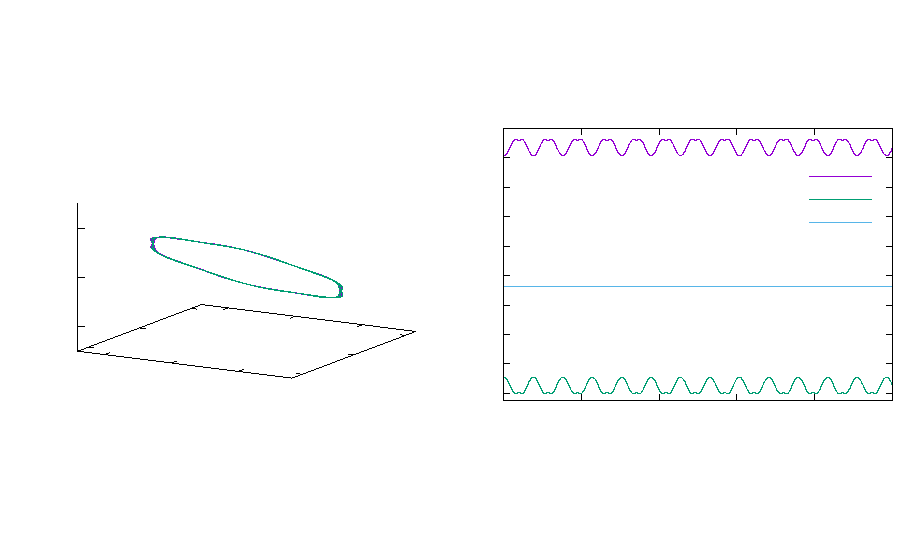
\includegraphics{MDSLP1}}%
    \gplfronttext
  \end{picture}%
\endgroup

	\caption{Trajectories (left) and plot of the kinetic, potential and total energy (right) for a system with $ N = 2 $ particles.
		\todo{replace gnuplot by python and add background grid to 3D plot}}
	\label{fig:MDSLP1}
\end{figure}

\section{Problem 2}
The trajectories and energy plots of a system with $ N = 3 $ particles is shown in \cref{fig:MDSLP2}.
\begin{figure}[h!]
	\centering
	% GNUPLOT: LaTeX picture with Postscript
\begingroup
  \makeatletter
  \providecommand\color[2][]{%
    \GenericError{(gnuplot) \space\space\space\@spaces}{%
      Package color not loaded in conjunction with
      terminal option `colourtext'%
    }{See the gnuplot documentation for explanation.%
    }{Either use 'blacktext' in gnuplot or load the package
      color.sty in LaTeX.}%
    \renewcommand\color[2][]{}%
  }%
  \providecommand\includegraphics[2][]{%
    \GenericError{(gnuplot) \space\space\space\@spaces}{%
      Package graphicx or graphics not loaded%
    }{See the gnuplot documentation for explanation.%
    }{The gnuplot epslatex terminal needs graphicx.sty or graphics.sty.}%
    \renewcommand\includegraphics[2][]{}%
  }%
  \providecommand\rotatebox[2]{#2}%
  \@ifundefined{ifGPcolor}{%
    \newif\ifGPcolor
    \GPcolorfalse
  }{}%
  \@ifundefined{ifGPblacktext}{%
    \newif\ifGPblacktext
    \GPblacktexttrue
  }{}%
  % define a \g@addto@macro without @ in the name:
  \let\gplgaddtomacro\g@addto@macro
  % define empty templates for all commands taking text:
  \gdef\gplbacktext{}%
  \gdef\gplfronttext{}%
  \makeatother
  \ifGPblacktext
    % no textcolor at all
    \def\colorrgb#1{}%
    \def\colorgray#1{}%
  \else
    % gray or color?
    \ifGPcolor
      \def\colorrgb#1{\color[rgb]{#1}}%
      \def\colorgray#1{\color[gray]{#1}}%
      \expandafter\def\csname LTw\endcsname{\color{white}}%
      \expandafter\def\csname LTb\endcsname{\color{black}}%
      \expandafter\def\csname LTa\endcsname{\color{black}}%
      \expandafter\def\csname LT0\endcsname{\color[rgb]{1,0,0}}%
      \expandafter\def\csname LT1\endcsname{\color[rgb]{0,1,0}}%
      \expandafter\def\csname LT2\endcsname{\color[rgb]{0,0,1}}%
      \expandafter\def\csname LT3\endcsname{\color[rgb]{1,0,1}}%
      \expandafter\def\csname LT4\endcsname{\color[rgb]{0,1,1}}%
      \expandafter\def\csname LT5\endcsname{\color[rgb]{1,1,0}}%
      \expandafter\def\csname LT6\endcsname{\color[rgb]{0,0,0}}%
      \expandafter\def\csname LT7\endcsname{\color[rgb]{1,0.3,0}}%
      \expandafter\def\csname LT8\endcsname{\color[rgb]{0.5,0.5,0.5}}%
    \else
      % gray
      \def\colorrgb#1{\color{black}}%
      \def\colorgray#1{\color[gray]{#1}}%
      \expandafter\def\csname LTw\endcsname{\color{white}}%
      \expandafter\def\csname LTb\endcsname{\color{black}}%
      \expandafter\def\csname LTa\endcsname{\color{black}}%
      \expandafter\def\csname LT0\endcsname{\color{black}}%
      \expandafter\def\csname LT1\endcsname{\color{black}}%
      \expandafter\def\csname LT2\endcsname{\color{black}}%
      \expandafter\def\csname LT3\endcsname{\color{black}}%
      \expandafter\def\csname LT4\endcsname{\color{black}}%
      \expandafter\def\csname LT5\endcsname{\color{black}}%
      \expandafter\def\csname LT6\endcsname{\color{black}}%
      \expandafter\def\csname LT7\endcsname{\color{black}}%
      \expandafter\def\csname LT8\endcsname{\color{black}}%
    \fi
  \fi
    \setlength{\unitlength}{0.0500bp}%
    \ifx\gptboxheight\undefined%
      \newlength{\gptboxheight}%
      \newlength{\gptboxwidth}%
      \newsavebox{\gptboxtext}%
    \fi%
    \setlength{\fboxrule}{0.5pt}%
    \setlength{\fboxsep}{1pt}%
\begin{picture}(8496.00,3528.00)%
    \gplgaddtomacro\gplbacktext{%
      \csname LTb\endcsname%
      \put(663,916){\makebox(0,0){\strut{}$-0.5$}}%
      \put(1131,857){\makebox(0,0){\strut{}$0$}}%
      \put(1599,798){\makebox(0,0){\strut{}$0.5$}}%
      \put(2067,739){\makebox(0,0){\strut{}$1$}}%
      \put(2534,681){\makebox(0,0){\strut{}$1.5$}}%
      \put(2879,763){\makebox(0,0){\strut{}$-0.5$}}%
      \put(3149,864){\makebox(0,0){\strut{}$0$}}%
      \put(3420,966){\makebox(0,0){\strut{}$0.5$}}%
      \put(3690,1068){\makebox(0,0){\strut{}$1$}}%
      \put(3960,1170){\makebox(0,0){\strut{}$1.5$}}%
      \put(459,1069){\makebox(0,0)[r]{\strut{}$-0.6$}}%
      \put(459,1272){\makebox(0,0)[r]{\strut{}$-0.4$}}%
      \put(459,1475){\makebox(0,0)[r]{\strut{}$-0.2$}}%
      \put(459,1678){\makebox(0,0)[r]{\strut{}$0$}}%
      \put(459,1880){\makebox(0,0)[r]{\strut{}$0.2$}}%
      \put(459,2083){\makebox(0,0)[r]{\strut{}$0.4$}}%
      \put(459,2286){\makebox(0,0)[r]{\strut{}$0.6$}}%
      \put(459,2489){\makebox(0,0)[r]{\strut{}$0.8$}}%
      \put(-75,1780){\makebox(0,0){\strut{}z}}%
    }%
    \gplgaddtomacro\gplfronttext{%
      \csname LTb\endcsname%
      \put(1318,609){\makebox(0,0){\strut{}x}}%
      \put(3753,751){\makebox(0,0){\strut{}y}}%
      \put(-75,1780){\makebox(0,0){\strut{}z}}%
    }%
    \gplgaddtomacro\gplbacktext{%
      \csname LTb\endcsname%
      \put(4540,593){\makebox(0,0)[r]{\strut{}$-3$}}%
      \put(4540,855){\makebox(0,0)[r]{\strut{}$-2.5$}}%
      \put(4540,1116){\makebox(0,0)[r]{\strut{}$-2$}}%
      \put(4540,1378){\makebox(0,0)[r]{\strut{}$-1.5$}}%
      \put(4540,1639){\makebox(0,0)[r]{\strut{}$-1$}}%
      \put(4540,1901){\makebox(0,0)[r]{\strut{}$-0.5$}}%
      \put(4540,2163){\makebox(0,0)[r]{\strut{}$0$}}%
      \put(4540,2424){\makebox(0,0)[r]{\strut{}$0.5$}}%
      \put(4540,2686){\makebox(0,0)[r]{\strut{}$1$}}%
      \put(4540,2947){\makebox(0,0)[r]{\strut{}$1.5$}}%
      \put(4540,3209){\makebox(0,0)[r]{\strut{}$2$}}%
      \put(4672,373){\makebox(0,0){\strut{}$0$}}%
      \put(5420,373){\makebox(0,0){\strut{}$2$}}%
      \put(6167,373){\makebox(0,0){\strut{}$4$}}%
      \put(6915,373){\makebox(0,0){\strut{}$6$}}%
      \put(7662,373){\makebox(0,0){\strut{}$8$}}%
      \put(8410,373){\makebox(0,0){\strut{}$10$}}%
    }%
    \gplgaddtomacro\gplfronttext{%
      \csname LTb\endcsname%
      \put(3968,1901){\rotatebox{-270}{\makebox(0,0){\strut{}energy}}}%
      \put(6541,208){\makebox(0,0){\strut{}time t}}%
      \csname LTb\endcsname%
      \put(7480,2210){\makebox(0,0)[r]{\strut{}Kinetic energy}}%
      \csname LTb\endcsname%
      \put(7480,1990){\makebox(0,0)[r]{\strut{}Potential energy}}%
      \csname LTb\endcsname%
      \put(7480,1770){\makebox(0,0)[r]{\strut{}Total energy}}%
    }%
    \gplbacktext
    \put(0,0){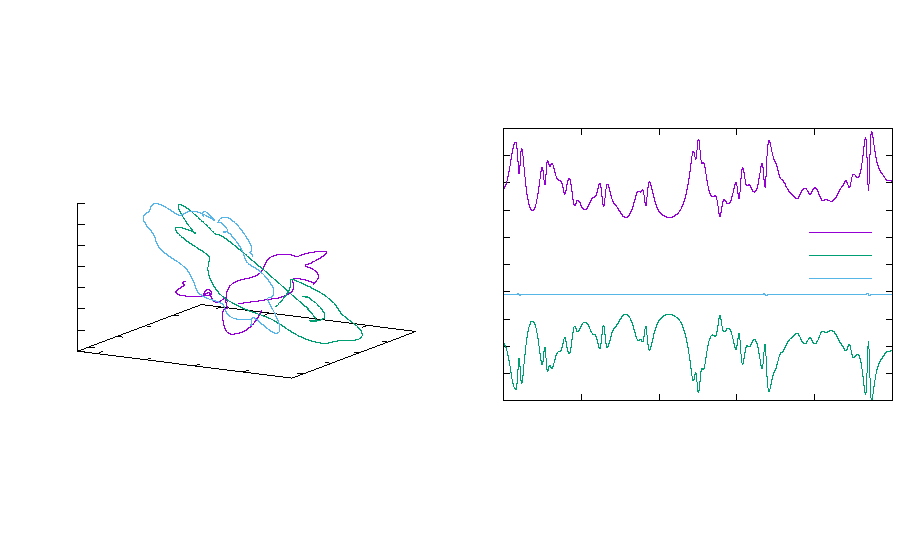
\includegraphics{MDSLP2}}%
    \gplfronttext
  \end{picture}%
\endgroup

	\caption{Trajectories (left) and plot of the kinetic, potential and total energy (right) for a system with $ N = 3 $ particles.}
	\label{fig:MDSLP2}
\end{figure}

\section{Problem 3}
The trajectories and energy plots of systems with $ N = 4 $, $ N = 5 $ and $ N = 6 $ are shown in \cref{fig:MDSLP3N4,fig:MDSLP3N5,fig:MDSLP3N6}.

\begin{figure}[h!]
	\centering
	% GNUPLOT: LaTeX picture with Postscript
\begingroup
  \makeatletter
  \providecommand\color[2][]{%
    \GenericError{(gnuplot) \space\space\space\@spaces}{%
      Package color not loaded in conjunction with
      terminal option `colourtext'%
    }{See the gnuplot documentation for explanation.%
    }{Either use 'blacktext' in gnuplot or load the package
      color.sty in LaTeX.}%
    \renewcommand\color[2][]{}%
  }%
  \providecommand\includegraphics[2][]{%
    \GenericError{(gnuplot) \space\space\space\@spaces}{%
      Package graphicx or graphics not loaded%
    }{See the gnuplot documentation for explanation.%
    }{The gnuplot epslatex terminal needs graphicx.sty or graphics.sty.}%
    \renewcommand\includegraphics[2][]{}%
  }%
  \providecommand\rotatebox[2]{#2}%
  \@ifundefined{ifGPcolor}{%
    \newif\ifGPcolor
    \GPcolorfalse
  }{}%
  \@ifundefined{ifGPblacktext}{%
    \newif\ifGPblacktext
    \GPblacktexttrue
  }{}%
  % define a \g@addto@macro without @ in the name:
  \let\gplgaddtomacro\g@addto@macro
  % define empty templates for all commands taking text:
  \gdef\gplbacktext{}%
  \gdef\gplfronttext{}%
  \makeatother
  \ifGPblacktext
    % no textcolor at all
    \def\colorrgb#1{}%
    \def\colorgray#1{}%
  \else
    % gray or color?
    \ifGPcolor
      \def\colorrgb#1{\color[rgb]{#1}}%
      \def\colorgray#1{\color[gray]{#1}}%
      \expandafter\def\csname LTw\endcsname{\color{white}}%
      \expandafter\def\csname LTb\endcsname{\color{black}}%
      \expandafter\def\csname LTa\endcsname{\color{black}}%
      \expandafter\def\csname LT0\endcsname{\color[rgb]{1,0,0}}%
      \expandafter\def\csname LT1\endcsname{\color[rgb]{0,1,0}}%
      \expandafter\def\csname LT2\endcsname{\color[rgb]{0,0,1}}%
      \expandafter\def\csname LT3\endcsname{\color[rgb]{1,0,1}}%
      \expandafter\def\csname LT4\endcsname{\color[rgb]{0,1,1}}%
      \expandafter\def\csname LT5\endcsname{\color[rgb]{1,1,0}}%
      \expandafter\def\csname LT6\endcsname{\color[rgb]{0,0,0}}%
      \expandafter\def\csname LT7\endcsname{\color[rgb]{1,0.3,0}}%
      \expandafter\def\csname LT8\endcsname{\color[rgb]{0.5,0.5,0.5}}%
    \else
      % gray
      \def\colorrgb#1{\color{black}}%
      \def\colorgray#1{\color[gray]{#1}}%
      \expandafter\def\csname LTw\endcsname{\color{white}}%
      \expandafter\def\csname LTb\endcsname{\color{black}}%
      \expandafter\def\csname LTa\endcsname{\color{black}}%
      \expandafter\def\csname LT0\endcsname{\color{black}}%
      \expandafter\def\csname LT1\endcsname{\color{black}}%
      \expandafter\def\csname LT2\endcsname{\color{black}}%
      \expandafter\def\csname LT3\endcsname{\color{black}}%
      \expandafter\def\csname LT4\endcsname{\color{black}}%
      \expandafter\def\csname LT5\endcsname{\color{black}}%
      \expandafter\def\csname LT6\endcsname{\color{black}}%
      \expandafter\def\csname LT7\endcsname{\color{black}}%
      \expandafter\def\csname LT8\endcsname{\color{black}}%
    \fi
  \fi
    \setlength{\unitlength}{0.0500bp}%
    \ifx\gptboxheight\undefined%
      \newlength{\gptboxheight}%
      \newlength{\gptboxwidth}%
      \newsavebox{\gptboxtext}%
    \fi%
    \setlength{\fboxrule}{0.5pt}%
    \setlength{\fboxsep}{1pt}%
\begin{picture}(8496.00,5040.00)%
    \gplgaddtomacro\gplbacktext{%
      \csname LTb\endcsname%
      \put(475,1695){\makebox(0,0){\strut{}$-2$}}%
      \put(770,1658){\makebox(0,0){\strut{}$-1$}}%
      \put(1064,1621){\makebox(0,0){\strut{}$0$}}%
      \put(1358,1584){\makebox(0,0){\strut{}$1$}}%
      \put(1652,1548){\makebox(0,0){\strut{}$2$}}%
      \put(1947,1511){\makebox(0,0){\strut{}$3$}}%
      \put(2240,1474){\makebox(0,0){\strut{}$4$}}%
      \put(2534,1437){\makebox(0,0){\strut{}$5$}}%
      \put(2771,1478){\makebox(0,0){\strut{}$-1$}}%
      \put(3068,1590){\makebox(0,0){\strut{}$0$}}%
      \put(3366,1702){\makebox(0,0){\strut{}$1$}}%
      \put(3663,1814){\makebox(0,0){\strut{}$2$}}%
      \put(3960,1926){\makebox(0,0){\strut{}$3$}}%
      \put(459,1983){\makebox(0,0)[r]{\strut{}$-2$}}%
      \put(459,2299){\makebox(0,0)[r]{\strut{}$-1$}}%
      \put(459,2615){\makebox(0,0)[r]{\strut{}$0$}}%
      \put(459,2930){\makebox(0,0)[r]{\strut{}$1$}}%
      \put(459,3245){\makebox(0,0)[r]{\strut{}$2$}}%
      \put(-75,2536){\makebox(0,0){\strut{}z}}%
    }%
    \gplgaddtomacro\gplfronttext{%
      \csname LTb\endcsname%
      \put(1318,1365){\makebox(0,0){\strut{}x}}%
      \put(3753,1507){\makebox(0,0){\strut{}y}}%
      \put(-75,2536){\makebox(0,0){\strut{}z}}%
    }%
    \gplgaddtomacro\gplbacktext{%
      \csname LTb\endcsname%
      \put(4540,1587){\makebox(0,0)[r]{\strut{}$-4$}}%
      \put(4540,1927){\makebox(0,0)[r]{\strut{}$-3$}}%
      \put(4540,2266){\makebox(0,0)[r]{\strut{}$-2$}}%
      \put(4540,2606){\makebox(0,0)[r]{\strut{}$-1$}}%
      \put(4540,2946){\makebox(0,0)[r]{\strut{}$0$}}%
      \put(4540,3286){\makebox(0,0)[r]{\strut{}$1$}}%
      \put(4540,3625){\makebox(0,0)[r]{\strut{}$2$}}%
      \put(4540,3965){\makebox(0,0)[r]{\strut{}$3$}}%
      \put(4672,1129){\makebox(0,0){\strut{}$0$}}%
      \put(5420,1129){\makebox(0,0){\strut{}$2$}}%
      \put(6167,1129){\makebox(0,0){\strut{}$4$}}%
      \put(6915,1129){\makebox(0,0){\strut{}$6$}}%
      \put(7662,1129){\makebox(0,0){\strut{}$8$}}%
      \put(8410,1129){\makebox(0,0){\strut{}$10$}}%
    }%
    \gplgaddtomacro\gplfronttext{%
      \csname LTb\endcsname%
      \put(4232,2657){\rotatebox{-270}{\makebox(0,0){\strut{}energy}}}%
      \put(6541,964){\makebox(0,0){\strut{}time t}}%
      \csname LTb\endcsname%
      \put(7480,3023){\makebox(0,0)[r]{\strut{}Kinetic energy}}%
      \csname LTb\endcsname%
      \put(7480,2803){\makebox(0,0)[r]{\strut{}Potential energy}}%
      \csname LTb\endcsname%
      \put(7480,2583){\makebox(0,0)[r]{\strut{}Total energy}}%
    }%
    \gplbacktext
    \put(0,0){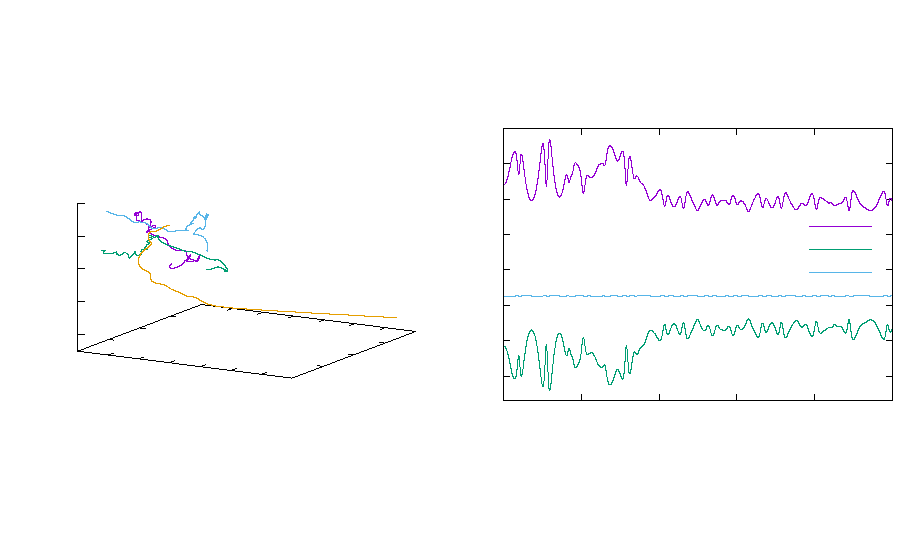
\includegraphics{MDSLP3N4}}%
    \gplfronttext
  \end{picture}%
\endgroup

	\caption{Trajectories (left) and plot of the kinetic, potential and total energy (right) for a system with $ N = 4 $ particles.}
	\label{fig:MDSLP3N4}
\end{figure}

\begin{figure}[h!]
	\centering
	% GNUPLOT: LaTeX picture with Postscript
\begingroup
  \makeatletter
  \providecommand\color[2][]{%
    \GenericError{(gnuplot) \space\space\space\@spaces}{%
      Package color not loaded in conjunction with
      terminal option `colourtext'%
    }{See the gnuplot documentation for explanation.%
    }{Either use 'blacktext' in gnuplot or load the package
      color.sty in LaTeX.}%
    \renewcommand\color[2][]{}%
  }%
  \providecommand\includegraphics[2][]{%
    \GenericError{(gnuplot) \space\space\space\@spaces}{%
      Package graphicx or graphics not loaded%
    }{See the gnuplot documentation for explanation.%
    }{The gnuplot epslatex terminal needs graphicx.sty or graphics.sty.}%
    \renewcommand\includegraphics[2][]{}%
  }%
  \providecommand\rotatebox[2]{#2}%
  \@ifundefined{ifGPcolor}{%
    \newif\ifGPcolor
    \GPcolorfalse
  }{}%
  \@ifundefined{ifGPblacktext}{%
    \newif\ifGPblacktext
    \GPblacktexttrue
  }{}%
  % define a \g@addto@macro without @ in the name:
  \let\gplgaddtomacro\g@addto@macro
  % define empty templates for all commands taking text:
  \gdef\gplbacktext{}%
  \gdef\gplfronttext{}%
  \makeatother
  \ifGPblacktext
    % no textcolor at all
    \def\colorrgb#1{}%
    \def\colorgray#1{}%
  \else
    % gray or color?
    \ifGPcolor
      \def\colorrgb#1{\color[rgb]{#1}}%
      \def\colorgray#1{\color[gray]{#1}}%
      \expandafter\def\csname LTw\endcsname{\color{white}}%
      \expandafter\def\csname LTb\endcsname{\color{black}}%
      \expandafter\def\csname LTa\endcsname{\color{black}}%
      \expandafter\def\csname LT0\endcsname{\color[rgb]{1,0,0}}%
      \expandafter\def\csname LT1\endcsname{\color[rgb]{0,1,0}}%
      \expandafter\def\csname LT2\endcsname{\color[rgb]{0,0,1}}%
      \expandafter\def\csname LT3\endcsname{\color[rgb]{1,0,1}}%
      \expandafter\def\csname LT4\endcsname{\color[rgb]{0,1,1}}%
      \expandafter\def\csname LT5\endcsname{\color[rgb]{1,1,0}}%
      \expandafter\def\csname LT6\endcsname{\color[rgb]{0,0,0}}%
      \expandafter\def\csname LT7\endcsname{\color[rgb]{1,0.3,0}}%
      \expandafter\def\csname LT8\endcsname{\color[rgb]{0.5,0.5,0.5}}%
    \else
      % gray
      \def\colorrgb#1{\color{black}}%
      \def\colorgray#1{\color[gray]{#1}}%
      \expandafter\def\csname LTw\endcsname{\color{white}}%
      \expandafter\def\csname LTb\endcsname{\color{black}}%
      \expandafter\def\csname LTa\endcsname{\color{black}}%
      \expandafter\def\csname LT0\endcsname{\color{black}}%
      \expandafter\def\csname LT1\endcsname{\color{black}}%
      \expandafter\def\csname LT2\endcsname{\color{black}}%
      \expandafter\def\csname LT3\endcsname{\color{black}}%
      \expandafter\def\csname LT4\endcsname{\color{black}}%
      \expandafter\def\csname LT5\endcsname{\color{black}}%
      \expandafter\def\csname LT6\endcsname{\color{black}}%
      \expandafter\def\csname LT7\endcsname{\color{black}}%
      \expandafter\def\csname LT8\endcsname{\color{black}}%
    \fi
  \fi
    \setlength{\unitlength}{0.0500bp}%
    \ifx\gptboxheight\undefined%
      \newlength{\gptboxheight}%
      \newlength{\gptboxwidth}%
      \newsavebox{\gptboxtext}%
    \fi%
    \setlength{\fboxrule}{0.5pt}%
    \setlength{\fboxsep}{1pt}%
\begin{picture}(8496.00,5040.00)%
    \gplgaddtomacro\gplbacktext{%
      \csname LTb\endcsname%
      \put(770,1658){\makebox(0,0){\strut{}$-1$}}%
      \put(1358,1584){\makebox(0,0){\strut{}$0$}}%
      \put(1947,1511){\makebox(0,0){\strut{}$1$}}%
      \put(2534,1437){\makebox(0,0){\strut{}$2$}}%
      \put(2771,1478){\makebox(0,0){\strut{}$-1$}}%
      \put(3167,1627){\makebox(0,0){\strut{}$0$}}%
      \put(3564,1777){\makebox(0,0){\strut{}$1$}}%
      \put(3960,1926){\makebox(0,0){\strut{}$2$}}%
      \put(459,1825){\makebox(0,0)[r]{\strut{}$-1$}}%
      \put(459,2231){\makebox(0,0)[r]{\strut{}$0$}}%
      \put(459,2636){\makebox(0,0)[r]{\strut{}$1$}}%
      \put(459,3042){\makebox(0,0)[r]{\strut{}$2$}}%
      \put(-75,2536){\makebox(0,0){\strut{}z}}%
    }%
    \gplgaddtomacro\gplfronttext{%
      \csname LTb\endcsname%
      \put(1318,1365){\makebox(0,0){\strut{}x}}%
      \put(3753,1507){\makebox(0,0){\strut{}y}}%
      \put(-75,2536){\makebox(0,0){\strut{}z}}%
    }%
    \gplgaddtomacro\gplbacktext{%
      \csname LTb\endcsname%
      \put(4540,1587){\makebox(0,0)[r]{\strut{}$-6$}}%
      \put(4540,2062){\makebox(0,0)[r]{\strut{}$-4$}}%
      \put(4540,2538){\makebox(0,0)[r]{\strut{}$-2$}}%
      \put(4540,3014){\makebox(0,0)[r]{\strut{}$0$}}%
      \put(4540,3489){\makebox(0,0)[r]{\strut{}$2$}}%
      \put(4540,3965){\makebox(0,0)[r]{\strut{}$4$}}%
      \put(4672,1129){\makebox(0,0){\strut{}$0$}}%
      \put(5420,1129){\makebox(0,0){\strut{}$2$}}%
      \put(6167,1129){\makebox(0,0){\strut{}$4$}}%
      \put(6915,1129){\makebox(0,0){\strut{}$6$}}%
      \put(7662,1129){\makebox(0,0){\strut{}$8$}}%
      \put(8410,1129){\makebox(0,0){\strut{}$10$}}%
    }%
    \gplgaddtomacro\gplfronttext{%
      \csname LTb\endcsname%
      \put(4232,2657){\rotatebox{-270}{\makebox(0,0){\strut{}energy}}}%
      \put(6541,964){\makebox(0,0){\strut{}time t}}%
      \csname LTb\endcsname%
      \put(7480,3035){\makebox(0,0)[r]{\strut{}Kinetic energy}}%
      \csname LTb\endcsname%
      \put(7480,2815){\makebox(0,0)[r]{\strut{}Potential energy}}%
      \csname LTb\endcsname%
      \put(7480,2595){\makebox(0,0)[r]{\strut{}Total energy}}%
    }%
    \gplbacktext
    \put(0,0){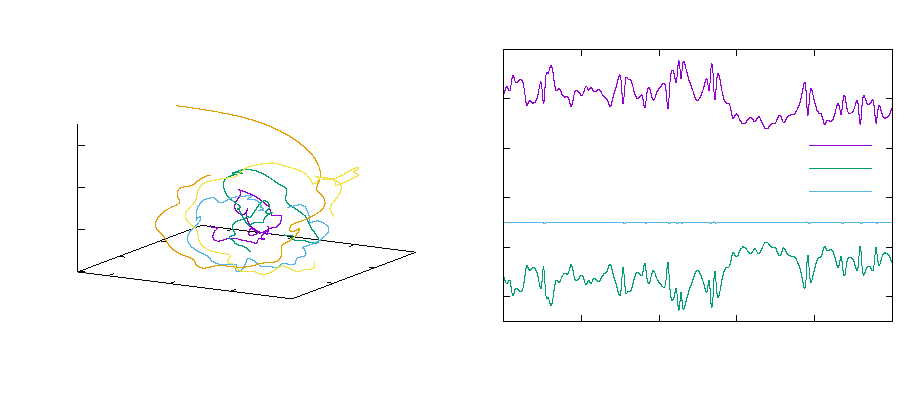
\includegraphics{MDSLP3N5}}%
    \gplfronttext
  \end{picture}%
\endgroup

	\caption{Trajectories (left) and plot of the kinetic, potential and total energy (right) for a system with $ N = 5 $ particles.}
	\label{fig:MDSLP3N5}
\end{figure}

\begin{figure}[h!]
	\centering
	% GNUPLOT: LaTeX picture with Postscript
\begingroup
  \makeatletter
  \providecommand\color[2][]{%
    \GenericError{(gnuplot) \space\space\space\@spaces}{%
      Package color not loaded in conjunction with
      terminal option `colourtext'%
    }{See the gnuplot documentation for explanation.%
    }{Either use 'blacktext' in gnuplot or load the package
      color.sty in LaTeX.}%
    \renewcommand\color[2][]{}%
  }%
  \providecommand\includegraphics[2][]{%
    \GenericError{(gnuplot) \space\space\space\@spaces}{%
      Package graphicx or graphics not loaded%
    }{See the gnuplot documentation for explanation.%
    }{The gnuplot epslatex terminal needs graphicx.sty or graphics.sty.}%
    \renewcommand\includegraphics[2][]{}%
  }%
  \providecommand\rotatebox[2]{#2}%
  \@ifundefined{ifGPcolor}{%
    \newif\ifGPcolor
    \GPcolorfalse
  }{}%
  \@ifundefined{ifGPblacktext}{%
    \newif\ifGPblacktext
    \GPblacktexttrue
  }{}%
  % define a \g@addto@macro without @ in the name:
  \let\gplgaddtomacro\g@addto@macro
  % define empty templates for all commands taking text:
  \gdef\gplbacktext{}%
  \gdef\gplfronttext{}%
  \makeatother
  \ifGPblacktext
    % no textcolor at all
    \def\colorrgb#1{}%
    \def\colorgray#1{}%
  \else
    % gray or color?
    \ifGPcolor
      \def\colorrgb#1{\color[rgb]{#1}}%
      \def\colorgray#1{\color[gray]{#1}}%
      \expandafter\def\csname LTw\endcsname{\color{white}}%
      \expandafter\def\csname LTb\endcsname{\color{black}}%
      \expandafter\def\csname LTa\endcsname{\color{black}}%
      \expandafter\def\csname LT0\endcsname{\color[rgb]{1,0,0}}%
      \expandafter\def\csname LT1\endcsname{\color[rgb]{0,1,0}}%
      \expandafter\def\csname LT2\endcsname{\color[rgb]{0,0,1}}%
      \expandafter\def\csname LT3\endcsname{\color[rgb]{1,0,1}}%
      \expandafter\def\csname LT4\endcsname{\color[rgb]{0,1,1}}%
      \expandafter\def\csname LT5\endcsname{\color[rgb]{1,1,0}}%
      \expandafter\def\csname LT6\endcsname{\color[rgb]{0,0,0}}%
      \expandafter\def\csname LT7\endcsname{\color[rgb]{1,0.3,0}}%
      \expandafter\def\csname LT8\endcsname{\color[rgb]{0.5,0.5,0.5}}%
    \else
      % gray
      \def\colorrgb#1{\color{black}}%
      \def\colorgray#1{\color[gray]{#1}}%
      \expandafter\def\csname LTw\endcsname{\color{white}}%
      \expandafter\def\csname LTb\endcsname{\color{black}}%
      \expandafter\def\csname LTa\endcsname{\color{black}}%
      \expandafter\def\csname LT0\endcsname{\color{black}}%
      \expandafter\def\csname LT1\endcsname{\color{black}}%
      \expandafter\def\csname LT2\endcsname{\color{black}}%
      \expandafter\def\csname LT3\endcsname{\color{black}}%
      \expandafter\def\csname LT4\endcsname{\color{black}}%
      \expandafter\def\csname LT5\endcsname{\color{black}}%
      \expandafter\def\csname LT6\endcsname{\color{black}}%
      \expandafter\def\csname LT7\endcsname{\color{black}}%
      \expandafter\def\csname LT8\endcsname{\color{black}}%
    \fi
  \fi
    \setlength{\unitlength}{0.0500bp}%
    \ifx\gptboxheight\undefined%
      \newlength{\gptboxheight}%
      \newlength{\gptboxwidth}%
      \newsavebox{\gptboxtext}%
    \fi%
    \setlength{\fboxrule}{0.5pt}%
    \setlength{\fboxsep}{1pt}%
\begin{picture}(8496.00,3528.00)%
    \gplgaddtomacro\gplbacktext{%
      \csname LTb\endcsname%
      \put(819,896){\makebox(0,0){\strut{}$0$}}%
      \put(1505,810){\makebox(0,0){\strut{}$1$}}%
      \put(2192,724){\makebox(0,0){\strut{}$2$}}%
      \put(2771,722){\makebox(0,0){\strut{}$-1$}}%
      \put(3167,871){\makebox(0,0){\strut{}$0$}}%
      \put(3564,1021){\makebox(0,0){\strut{}$1$}}%
      \put(3960,1170){\makebox(0,0){\strut{}$2$}}%
      \put(459,1069){\makebox(0,0)[r]{\strut{}$-1$}}%
      \put(459,1475){\makebox(0,0)[r]{\strut{}$0$}}%
      \put(459,1880){\makebox(0,0)[r]{\strut{}$1$}}%
      \put(459,2286){\makebox(0,0)[r]{\strut{}$2$}}%
      \put(-75,1780){\makebox(0,0){\strut{}z}}%
    }%
    \gplgaddtomacro\gplfronttext{%
      \csname LTb\endcsname%
      \put(1318,609){\makebox(0,0){\strut{}x}}%
      \put(3753,751){\makebox(0,0){\strut{}y}}%
      \put(-75,1780){\makebox(0,0){\strut{}z}}%
    }%
    \gplgaddtomacro\gplbacktext{%
      \csname LTb\endcsname%
      \put(4540,747){\makebox(0,0)[r]{\strut{}$-10$}}%
      \put(4540,1055){\makebox(0,0)[r]{\strut{}$-8$}}%
      \put(4540,1362){\makebox(0,0)[r]{\strut{}$-6$}}%
      \put(4540,1670){\makebox(0,0)[r]{\strut{}$-4$}}%
      \put(4540,1978){\makebox(0,0)[r]{\strut{}$-2$}}%
      \put(4540,2286){\makebox(0,0)[r]{\strut{}$0$}}%
      \put(4540,2593){\makebox(0,0)[r]{\strut{}$2$}}%
      \put(4540,2901){\makebox(0,0)[r]{\strut{}$4$}}%
      \put(4540,3209){\makebox(0,0)[r]{\strut{}$6$}}%
      \put(4672,373){\makebox(0,0){\strut{}$0$}}%
      \put(5420,373){\makebox(0,0){\strut{}$2$}}%
      \put(6167,373){\makebox(0,0){\strut{}$4$}}%
      \put(6915,373){\makebox(0,0){\strut{}$6$}}%
      \put(7662,373){\makebox(0,0){\strut{}$8$}}%
      \put(8410,373){\makebox(0,0){\strut{}$10$}}%
    }%
    \gplgaddtomacro\gplfronttext{%
      \csname LTb\endcsname%
      \put(4100,1901){\rotatebox{-270}{\makebox(0,0){\strut{}energy}}}%
      \put(6541,208){\makebox(0,0){\strut{}time t}}%
      \csname LTb\endcsname%
      \put(7480,2260){\makebox(0,0)[r]{\strut{}Kinetic energy}}%
      \csname LTb\endcsname%
      \put(7480,2040){\makebox(0,0)[r]{\strut{}Potential energy}}%
      \csname LTb\endcsname%
      \put(7480,1820){\makebox(0,0)[r]{\strut{}Total energy}}%
    }%
    \gplbacktext
    \put(0,0){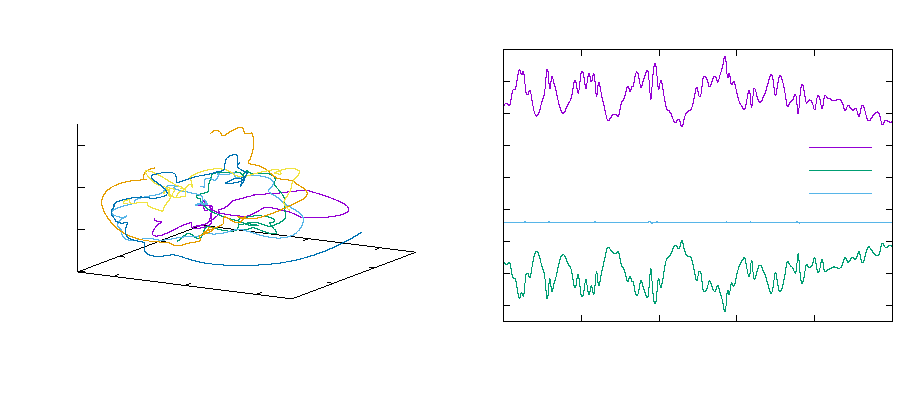
\includegraphics{MDSLP3N6}}%
    \gplfronttext
  \end{picture}%
\endgroup

	\caption{Trajectories (left) and plot of the kinetic, potential and total energy (right) for a system with $ N = 6 $ particles.}
	\label{fig:MDSLP3N6}
\end{figure}

\section{Problem 4}
\todo{Problem 4 maken}

\section{Problem 5}
\todo{Problem 5 maken}

\section{Problem 6}
\todo{Problem 6 maken}

\section{Problem 7}
\todo{Problem 7 maken}

\section{Problem 8}
\todo{Problem 8 maken}

\section{Problem 9}
\todo{Problem 9 maken}

\section{Master exercise}
\todo[inline]{choose 1 of the master exercises}

\insertbibliography
%\begin{appendices}
%% appendices hier
%
%
%\end{appendices}


\end{document}